
%----------------------------------------------------------------------------------------


%%%%%%%%%%%%%%% Za a5 format
\documentclass[10pt]{book}
\usepackage[a4paper,top=2.5cm, bottom=2cm, left = 2.5cm, right=2cm, twoside=true]{geometry}
%%%%%%%%%%%%%% Za 
%\documentclass[12pt]{report}
%\usepackage{geometry}
% \geometry{
% a4paper,
% total={165mm,237mm},
% left=25mm,
% top=30mm,
% }
%%%%%%%%%%%%%%%%%%%%%%%%%%%%%%%%

\usepackage[version=3]{mhchem} % Package for chemical equation typesetting
\usepackage{siunitx} % Provides the \SI{}{} and \si{} command for typesetting SI units
\usepackage{graphicx} % Required for the inclusion of images

\usepackage{natbib} % Required to change bibliography style to APA
\usepackage{amsmath} % Required for some math elements 
\usepackage{amssymb}

\usepackage[document]{ragged2e}  %%  za obostrano poravnanje

\setlength\parindent{0pt} % Removes all indentation from paragraphs

\usepackage{wrapfig} % Allows in-line images such as the example fish picture

%\renewcommand{\labelenumi}{\alph{enumi}.} % Make numbering in the enumerate environment by letter rather than number (e.g. section 6)

%%%%%%%%%%%%%%%%%%%%%%%%%%%%%%%%%%%%%%%%%%%%%%%%%%%%%%%%%%%%%%%%%%%%%%%%%%%%%%%%%%%%%%%%%%%%%%%%%%%%%%%%%%%%%%%%%%%%%%%%%%%%%%%%%%%
%%%%%%%%%%%%%%%%%%%%%%%%%%%%%%%%%%%%%%%%%%%%%%%%%%%     Lista
%%%%%%%%%%%%%%%%%%%%%%%%%%%%%%%%%%%%%%%%%%%%%%%%%%%%%%%%%%%%%%%%%%%%%%%%%%%%%%%%%%%%%%%%%%%%%%%%%%%%%%%%%%%%%%%%%%%%%%%%%%%%%%%%%%%

\usepackage{enumitem} % Customize lists
%\setlist{topsep=1.8mm,itemsep=0.01mm} % Moze se posebno definirati razmak izmedu redova i prvog reda
\setlist{nolistsep}  % Reduce spacing between bullet points and numbered lists

\usepackage{url} %% za printanje imena


\usepackage{setspace}  %% ovo je za razmak među redovima
%\onehalfspacing
%\doublespacing
\setstretch{1.0}

%%%%%%%%%%%%%%%%%%%%%%%%%%%%%%%%%%%%%%%%%%%%%%%%%%%%%%%%%%%%%%%%%%%%%%%%%%%%%%%%%%%%%%%%%%%%%%%%%%%%%%%%%%%%%%%%%%%%%%%%%%%%%%%%%%%
%%%%%%%%%%%%%%%%%%%%%%%%%%%%%%%%%%%%%%%%%%%%%%%%%%%     Brojaci
%%%%%%%%%%%%%%%%%%%%%%%%%%%%%%%%%%%%%%%%%%%%%%%%%%%%%%%%%%%%%%%%%%%%%%%%%%%%%%%%%%%%%%%%%%%%%%%%%%%%%%%%%%%%%%%%%%%%%%%%%%%%%%%%%%%
\newcounter{zadatak} %%%% Brojac
\newcounter{cjelina}
\setcounter{cjelina}{1}  %%%%%   Mjenjati ovisno o listu   !!!!!!!!!!!!!!!!!!!!!!!!!!!!!!!!!!!!!!!!!!!!!!!!!!!!!!
%\setcounter{}


%%%%%%%%%%%%%%%%%%%%%%%%%%%%%%%%%%%%%%%%%%%%%%%%%%%%%%%%%%%%%%%%%%%%%%%%%%%%%%%%%%%%%%%%%%%%%%%%%%%%%%%%%%%%%%%%%%%%%%%%%%%%%%%%%%%
%%%%%%%%%%%%%%%%%%%%%%%%%%%%%%%%%%%%%%%%%%%%%%%%%%%     Lista
%%%%%%%%%%%%%%%%%%%%%%%%%%%%%%%%%%%%%%%%%%%%%%%%%%%%%%%%%%%%%%%%%%%%%%%%%%%%%%%%%%%%%%%%%%%%%%%%%%%%%%%%%%%%%%%%%%%%%%%%%%%%%%%%%%%

\usepackage{enumitem} % Customize lists
\setlist{itemsep=0.3pt} % Reduce spacing between bullet points and numbered lists


%%%%%%%%%%%%%%%%%%%%%%%%%%%%%%%%%%%%%%%%%%%%%%%%%%%%%%%%%%%%%%%%%%%%%%%%%%%%%%%%%%%%%%%%%%%%%%%%%%%%%%%%%%%%%%%%%%%%%%%%%%%%%%%%%%%
%%%%%%%%%%%%%%%%%%%%%%%%%%%%%%%%%%%%%%%%%%%%%%%%%%%     Font
%%%%%%%%%%%%%%%%%%%%%%%%%%%%%%%%%%%%%%%%%%%%%%%%%%%%%%%%%%%%%%%%%%%%%%%%%%%%%%%%%%%%%%%%%%%%%%%%%%%%%%%%%%%%%%%%%%%%%%%%%%%%%%%%%%%

\usepackage[croatian]{babel}
%\usepackage{avant} % Use the Avantgarde font for headings
%\usepackage{times} % Use the Times font for headings
%\usepackage{mathptmx} % Use the Adobe Times Roman as the default text font together with math symbols from the Sym­bol, Chancery and Com­puter Modern fonts

\usepackage{microtype} % Slightly tweak font spacing for aesthetics
\usepackage[utf8]{inputenc} % Required for including letters with accents  Ovo je za hr
\usepackage[T1]{fontenc} % Use 8-bit encoding that has 256 glyphs

\usepackage[]{scrpage2}
\usepackage[]{blindtext}
 \usepackage{titlesec}
%\pagestyle{scrheadings}
%\setheadsepline[\textwidth]{0.25pt}{}

%Options: Sonny, Lenny, Glenn, Conny, Rejne, Bjarne, Bjornstrup
\usepackage[Bjornstrup]{fncychap}

\usepackage{color}
%\definecolor{boja}{RGB}{50, 180, 50}
\definecolor{boja}{RGB}{192,192,192}
%----------------------------------------------------------------------------------------
%	DOCUMENT INFORMATION
%----------------------------------------------------------------------------------------
%\titleformat{\section}  {\normalfont\fontsize{12}{15}\bfseries}{\thesection}{1em}{}


\begin{document}


\begin{titlepage}

\newcommand{\HRule}{\rule{\linewidth}{0.5mm}} % Defines a new command for the horizontal lines, change thickness here

\center % Center everything on the page

\textsc{\Large Sveučilište u Zagrebu\\ Geotehnički fakultet}\\[1.0cm] % Name of your university/college
%\textsc{\Large Major Heading}\\[0.5cm] % Major heading such as course name
%\textsc{\large Minor Heading}\\[0.5cm] % Minor heading such as course title


\includegraphics{logo_gfv.png}\\[2.0cm] % Include a department/university logo - this will require the graphicx package


\HRule \\[0.4cm]
{ \huge \bfseries Zadaci s vježbi iz kolegija Fizika 1}\\[0.4cm] % Title of your document
\HRule \\[1.5cm]

\textsc{\large Akademska godina 2018./2019.}\\[0.5cm] % Minor heading such as course title

%{\large \today}\\[3cm] % Date, change the \today to a set date if you want to be precise
\justify
 
\begin{center}
\begin{minipage}{0.8\textwidth}
\begin{justify} 
\vspace{1.2cm}
\begin{center}
doc. dr. sc. Ivan Hip\\
dr. sc. Marko Petric\\
dr. sc. Davor Stanko
                     
\end{center}

\end{justify}
\end{minipage}\\[3cm]
\today
\end{center}


\end{titlepage}

\pagenumbering{roman}


\tableofcontents
 
\clearpage

\pagenumbering{arabic}

%%%%%%%%%%%%%%%%%
%\renewcommand\thesection{\arabic{section}} %%% to je za nurmiranje bez chapter 
%%%%%%%%%%%%%%
\chapter{MATEMATIČKI TEMELJI}



\section{Vektori}


%


\noindent 
\textbf{\stepcounter{zadatak}
\thecjelina.\thezadatak.}
Nacrtajte slijedeća tri vektora u $xy$-ravnini: $\vec{a}=\vec{i}+3\vec{j}$, 
$\vec{b}=-3\vec{i}-2\vec{j}$, 
$\vec{c}=2\vec{i}-3\vec{j}$ 
i izračunajte računski i grafički:
\begin{enumerate}[label=\alph*)]
 \item Nacrtajte sva tri vektora u $xy$-ravnini.
 \item Koja dva vektora su okomita? Provjerite!
 \item Izračunajte računski i grafički $\vec{a} + \vec{b}$.
 \item Izračunajte računski i grafički $\vec{b} - \vec{c} $.
% \item $\vec{a} + \vec{c} $
\end{enumerate}


\noindent
{\color{boja} \rule{\linewidth}{0.3mm} }
\begin{enumerate}[label=\alph*)]
    \item $\vec{a}\cdot \vec{b} =(\vec{i}+3\vec{j})\cdot(-3\vec{i}-2\vec{j})=-9$
    
    $\vec{a}\cdot \vec{c} =(\vec{i}+3\vec{j})\cdot(2\vec{i}-3\vec{j})=-7$
    
    $\vec{b}\cdot \vec{c} =(-3\vec{i}-2\vec{j})\cdot(2\vec{i}-3\vec{j})=0$
    
 \item $\vec{a} + \vec{b}= \vec{i}+3\vec{j}-3\vec{i}-2\vec{j}= -2\vec{i}+\vec{j}$
 \item $\vec{b} - \vec{c}=-3\vec{i}-2\vec{j}-(2\vec{i}-3\vec{j})=-5 \vec{i}+\vec{j}$
 
\end{enumerate}

\vspace{0.8cm}




\noindent 
\textbf{\stepcounter{zadatak}
\thecjelina.\thezadatak.}
Zadani su vektori $\vec{a}=\vec{i}-2\vec{j}+3\vec{k} $ 
i $\vec{b}= -\vec{i}+ 2\vec{j}+3\vec{k}  $. Izračunajte:
\begin{enumerate}[label=\alph*)]
 \item $\vec{a} \cdot \vec{b}  $
 \item Kut između vektora $\vec{a}$ i $\vec{b}$.
 \item $\arrowvert \vec{a} \times \vec{b}  \arrowvert$ 
 \item $\vec{c}= \vec{a} \times \vec{b}  $ 
 \item Izračunajte $ | \vec{c} |$, gdje je $\vec{c}=\vec{a} \times \vec{b}$ i usporedite s rezultatom c).
 \item $\vec{d}=\vec{b}\times\vec{a}$ i usporedite s rezultatom d).
\end{enumerate}

\noindent
{\color{boja} \rule{\linewidth}{0.3mm} }



\begin{enumerate}[label=\alph*)]
 \item $\vec{a} \cdot \vec{b}=a_xb_x+a_yb_y+a_zb_z=1\cdot(-1)+(-2)\cdot2+3\cdot3=4  $
 \item   $$\vec{a} \cdot \vec{b}=|\vec{a}| \cdot| \vec{b}|\cos\alpha \ \ \ \ \ \Rightarrow  \ \ \ \ \  \cos\alpha=\frac{\vec{a} \cdot \vec{b}}{|\vec{a}| \cdot| \vec{b}|}$$
 $|\vec{a}|=\sqrt{a_x^2+a_y^2+a_z^2}=\sqrt{1^2+(-2)^2+3^2}=\sqrt{14}$
 
 $|\vec{b}|=\sqrt{b_x^2+b_y^2+b_z^2}\sqrt{(-1)^2+2^2+3^2}=\sqrt{14}$
 $$\cos\alpha=\frac{4}{\sqrt{14}\cdot\sqrt{14}} \ \ \ \ \Rightarrow  \ \ \ \  \alpha=\arccos \left( \frac{4}{\sqrt{14} \cdot \sqrt{14}} \right) 
  \ \ \ \ \Rightarrow  \ \ \ \   \alpha=73,4^\circ$$
 
 
 
 \item $\arrowvert \vec{a} \times \vec{b}  \arrowvert =  |\vec{a}| \cdot| \vec{b}|\sin\alpha =\sqrt{14}\cdot\sqrt{14} \sin(73,4^\circ)   $
 $$\arrowvert \vec{a} \times \vec{b}  \arrowvert \approx 13,42$$
 
 
 \item $  \vec{c} =?$
 
 $$\vec{c}=\vec{a} \times \vec{b}=
 \begin{vmatrix}
  \vec{i} & \vec{j} & \vec{k} \\
  a_x  & a_y  & a_z  \\
  b_x  & b_y  & b_z  \\
 \end{vmatrix}
 =\vec{i}(a_yb_z-a_zb_y)-\vec{j}(a_xb_z-a_zb_x) + \vec{k}(a_xb_y-a_yb_x)
 $$
 
 $$\vec{c}=
 \begin{vmatrix}
   \vec{i} & \vec{j} & \vec{k} \\
   1 & -2 & 3 \\
   -1 & 2 & 3 \\
 \end{vmatrix}
 =\vec{i}(-6-6)-\vec{j}(3-(-3))+ \vec{k}(2-2) $$
  $$\vec{c}= -12\vec{i}-6\vec{j} + 0\vec{k}$$
 \item 
 $$\vec{c}= -12\vec{i}-6\vec{j}  \ \ \ \ \Rightarrow  \ \ \ \ |\vec{c}|=\sqrt{144+36} \ \ \ \ \Rightarrow  \ \ \ \ |\vec{c}|\approx13,42 $$
 \item 
 $$\vec{d}=
 \begin{vmatrix}
   \vec{i} & \vec{j} & \vec{k} \\
   -1 & 2 & 3 \\
   1 & -2 & 3 \\
 \end{vmatrix}
 =\vec{i}(6+6)-\vec{j}(-3-3)+ \vec{k}(2-2) $$
  $$\vec{c}= 12\vec{i}+6\vec{j} + 0\vec{k}$$

\end{enumerate}


\section{Mjerne jedinice}
%To ćemo trebati za provjeru imena zadatka i oznake:
%\path{Matematicki_temelji/Zadatak_M802}


\noindent 
\textbf{\stepcounter{zadatak}
\thecjelina.\thezadatak.}
Pretvorite mjerene jedinice:
%\renewcommand{\labelenumii}{\Roman{enumii}} 
\begin{enumerate}[label=\alph*)]
  \item $0,1746\ rad=$ \hspace{2cm} $ ^\circ $
  \item $18,3\ MJ =$ \hspace{1.5cm} $ J$
  \item $0,016\ kN =$ \hspace{1.5cm} $ mN$  
  \item $100\ \mu g= $ \hspace{1.5cm} $ kg$
  \item $8,2\ kmh^{-1} =$ \hspace{1.5cm} $ms^{-1}$
  \item $36\ dana =$ \hspace{1.5cm} $min $
  \item $2\ cm^2=$ \hspace{1.5cm} $m^2 $
  \item $10\ L =$ \hspace{1.5cm} $m^3$
\end{enumerate}



\vspace{0.2cm}
\noindent
{\color{boja} \rule{\linewidth}{0.3mm} }

%\path{Matematicki_temelji/Rjesenje_M802}


\begin{enumerate}[label=\alph*)]
  \item $0,1746\ rad= 0,1746\ rad\ \frac{180 ^\circ}{\pi\ rad} = 10,00^\circ$ 
%  Proširimo sa jedinicom $1=180 ^\circ / \pi\ rad$ i poslije kraćenja 
%  mjerne jedinice $rad$ pomnožimo. 
%  \item  $57.5 ^\circ = 57.5^\circ\ \frac{\pi \ rad}{180^\circ}= 1.00\ rad$
  \item $0,016\ kN =1,6\cdot 10^{-2}\cdot 10^{3} N=1,6\cdot 10^1 N=$
  
  $=1,6\cdot 10^1 \cdot 10^{3}\cdot 10^{-3}N=1.6\cdot10^4 \ mN$
  \item $18,3\ MJ =1,83\cdot 10^1 \cdot 10^6\ J= 1,83\cdot 10^7\ J$
  \item $100\ \mu g= 10^2\cdot 10^{-6}\ g= 10^{-4}\ g=$
  
  $=10^{-4}\cdot 10^{-3}\cdot 10^3 \ g= 10^{-7}\ kg$
  \item $8,2\ kmh^{-1} =8,2 \frac{1000m}{3600s}=\frac{82}{36}\ ms^{-1}=2,28\ ms^{-1}  $
  \item $36\ dana =36\cdot24 \ h=36\cdot24\cdot60\ min = 51840 \ min$
  \item $2\ cm^2= 2\ (cm)^2=2\ (10^{-2}m)^2=2\cdot10^{-4}m^2=0,0002\ m^2 $
  \item $10\ L =10\ dm^3=10\ (dm)^3=10\ (10^{-1}m)^3=10\cdot 10^{-3}\  m^3=10^{-2}\ m^3=0.01\ m^3 $
\end{enumerate}

\vspace{0.8cm} 

\newpage
\chapter{KINEMATIKA MATERIJALNE TOČKE}
\stepcounter{cjelina} 
\setcounter{zadatak}{0}




\noindent 
\textbf{\stepcounter{zadatak}
\thecjelina.\thezadatak.}
Gibanje materijalne točke (MT) opisano je vektorom položaja
$$
\vec{r}(t)=(v_0 t)\vec{j} +(z_0 -\frac{1}{2}gt^2)\vec{k}.
$$
U trenutku $t=0\ s$ MT se nalazi na visini $z_0=80\ m$, a iznos početne brzine je $v_0=30\ ms^{-1}$.
Iznos ubrzanja slobodnog pada je $g=9,81\ ms^{-2}$, ali radi lakšek računanja može se uzeti približna vrijednost $g=10\ ms^{-2}$.
\begin{enumerate}[label=\alph*)]
  \item Izračunajte položaj MT svakih pola sekunde i skicirajte putanju u $yz$-ravnini.
  \item  Odredite vektor trenutne brzine $\vec{v}(t)$.
  \item Izračunajte i skicirajte trenutnu brzinu u trenucima $t_1=1\ s$, $t_2=2\ s$, $t_3=3\ s$ i $t_4=4\ s$.
  \item Odredite trenutno ubrzanje $\vec{a}(t)$ i skicirajte ga u nekoliko točaka putanje.
\end{enumerate}

%\vspace{0.2cm}
\noindent
{\color{boja} \rule{\linewidth}{0.3mm} }

Uvrstimo zadane vrijednosti u $\vec{r}(t)$.
$$
\vec{r}(t)=(30ms^{-1}t) \vec{j} +(80m-\frac{1}{2}10ms^{-2}t^2 )\vec{k}
$$

\begin{enumerate}[label=\alph*)]
  \item $ \vec{r}(t=0,0s)=(30ms^{-1}0s) \vec{j} +(80m-\frac{1}{2}10ms^{-2}(0s)^2 )\vec{k}= 0m\vec{j}+80m\vec{k}$
  
  $ \vec{r}(t=0,5s)=(30ms^{-1}0,5s) \vec{j} +(80m-\frac{1}{2}10ms^{-2}(0,5s)^2 )\vec{k}= 15m\vec{j}+78,75m\vec{k}$
  
  $ \vec{r}(t=1,0s)=(30ms^{-1}1,0s) \vec{j} +(80m-\frac{1}{2}10ms^{-2}(1,0s)^2 )\vec{k}= 30m\vec{j}+75m\vec{k}$
  
  $ \vec{r}(t=1,5s)=(30ms^{-1}1,5s) \vec{j} +(80m-\frac{1}{2}10ms^{-2}(1,5s)^2 )\vec{k}= 45m\vec{j}+68,75m\vec{k}$
  
  $ \vec{r}(t=2,0s)=(30ms^{-1}2,0s) \vec{j} +(80m-\frac{1}{2}10ms^{-2}(2,0s)^2 )\vec{k}= 60m\vec{j}+60m\vec{k}$
  
  $ \vec{r}(t=2,5s)=(30ms^{-1}2,5s) \vec{j} +(80m-\frac{1}{2}10ms^{-2}(2,5s)^2 )\vec{k}= 75m\vec{j}+48,75m\vec{k}$
   
  $ \vec{r}(t=3,0s)=(30ms^{-1}3,0s) \vec{j} +(80m-\frac{1}{2}10ms^{-2}(3,0s)^2 )\vec{k}= 90m\vec{j}+35m\vec{k}$
  
  $ \vec{r}(t=3,5s)=(30ms^{-1}3,5s) \vec{j} +(80m-\frac{1}{2}10ms^{-2}(3,5s)^2 )\vec{k}= 105m\vec{j}+18,75m\vec{k}$

  $ \vec{r}(t=4,0s)=(30ms^{-1}4,0s) \vec{j} +(80m-\frac{1}{2}10ms^{-2}(4,0s)^2 )\vec{k}= 120m\vec{j}+0m\vec{k}$

\begin{figure}
%\begin{subfigure}{.5\textwidth}
  \centering
  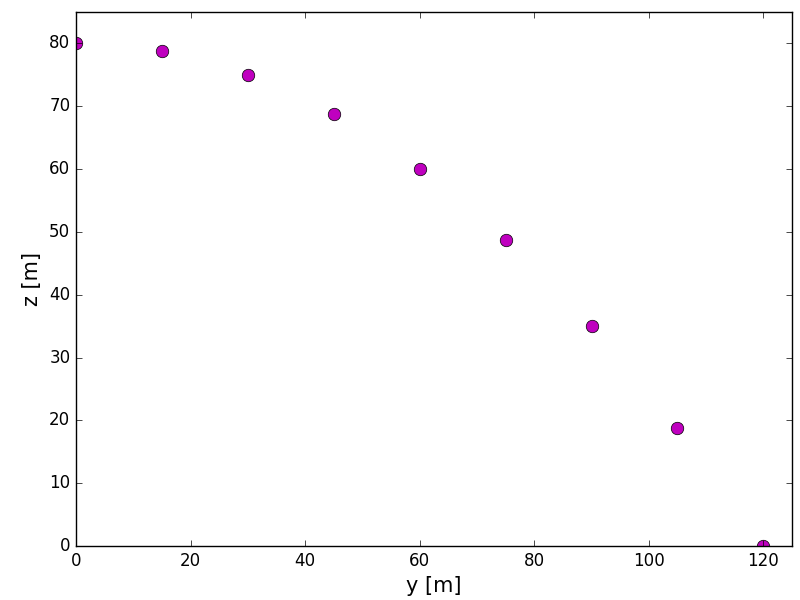
\includegraphics[width=0.5\linewidth]{Kinematika_materijalne_tocke/polozaj_MT.png}
%  \caption{1a}
%  \label{fig:sfig1}
%\end{subfigure}%
%\begin{subfigure}{.5\textwidth}
  \centering
  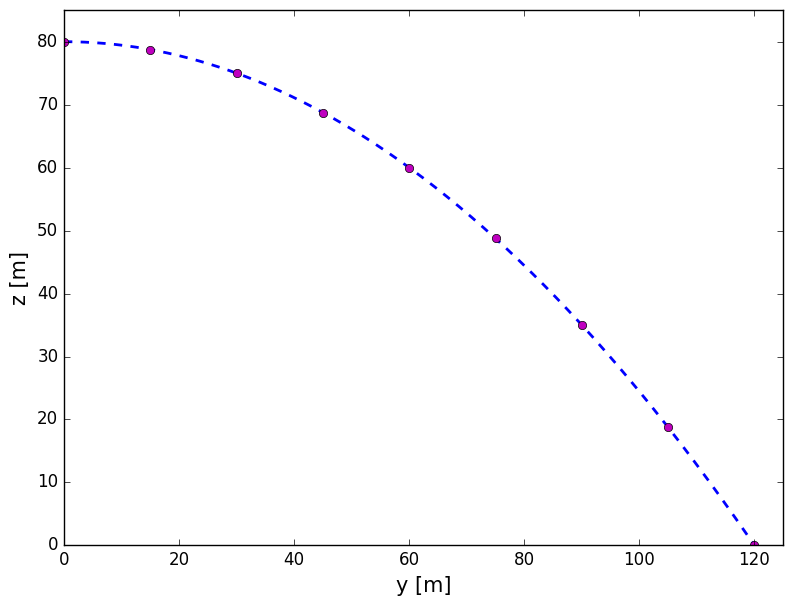
\includegraphics[width=.5\linewidth]{Kinematika_materijalne_tocke/krivulja_MT.png}
%  \caption{1b}
%  \label{fig:sfig2}
%\end{subfigure}
\caption{\textit{(lijevo)} Položaj MT za svakih $0,5\ s$. \textit{(desno)} Putanja MT do udarca o tlo.}
%\label{fig:poloza_MT}
\end{figure}
 
 
 
 \item $$\vec{v}(t)  = \frac{d\vec{r}(t)}{dt}$$
  
 $$\vec{v}(t)  = \frac{d}{dt} \left(z_0 \vec{k}+v_0t \vec{j}-\frac{1}{2}gt^2\vec{k}  \right)$$

 $$\vec{v}(t)  = v_0\vec{j}-gt\vec{k}$$
 
 \item $\vec{v}(t)  =30\ ms^{-1}\vec{j}-10\ ms^{-2}t\vec{k}$
 
 $\vec{v}(t=1s)  =30\ ms^{-1}\vec{j}-10\ ms^{-2}1s\vec{k}$
 
 $\vec{v}(t=1s)  =30\ ms^{-1}\vec{j}-10\ ms^{-1}\vec{k}$
 
 $\vec{v}(t=2s)  =30\ ms^{-1}\vec{j}-20\ ms^{-1}\vec{k}$
 
 $\vec{v}(t=3s)  =30\ ms^{-1}\vec{j}-30\ ms^{-1}\vec{k}$
  
 $\vec{v}(t=4s)  =30\ ms^{-1}\vec{j}-40\ ms^{-1}\vec{k}$
 
\begin{figure}
%\begin{subfigure}{.5\textwidth}
  \centering
  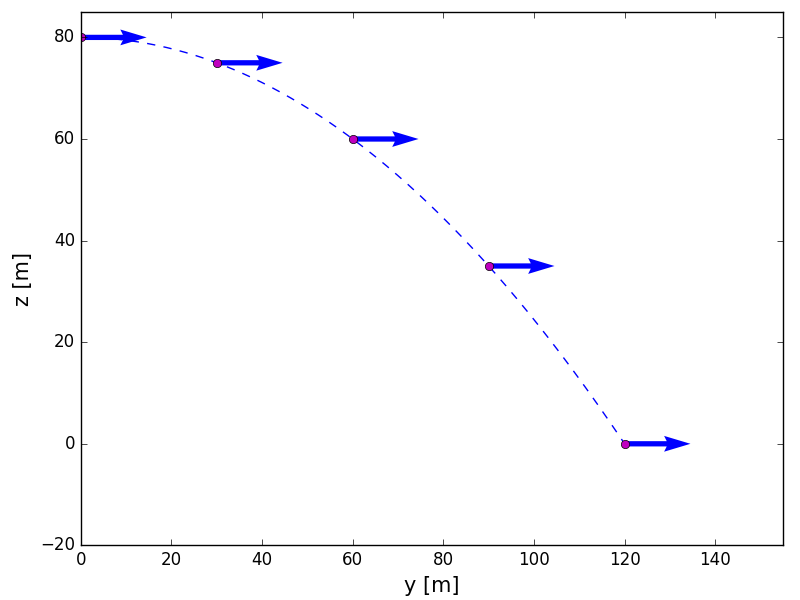
\includegraphics[width=0.4\linewidth]{Kinematika_materijalne_tocke/brzina_y.png}
%  \caption{1a}
%  \label{fig:sfig1}
%\end{subfigure}%
%\begin{subfigure}{.5\textwidth}
  \centering
  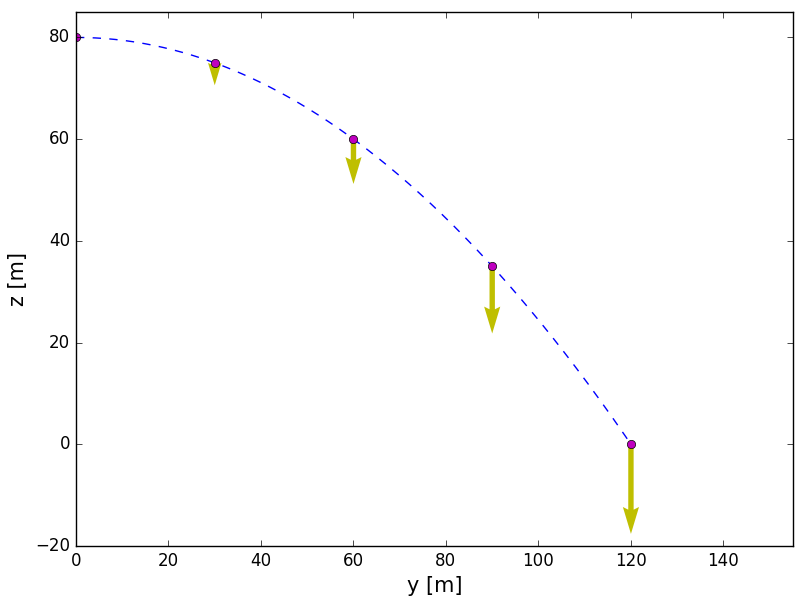
\includegraphics[width=.4\linewidth]{Kinematika_materijalne_tocke/brzina_z.png}
%  \caption{1b}
%  \label{fig:sfig2}
%\end{subfigure}
\centering
  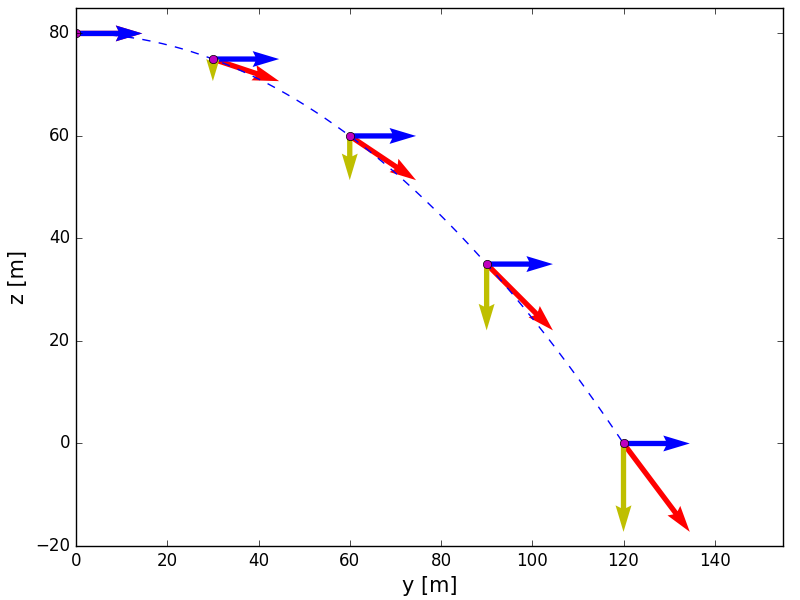
\includegraphics[width=.5\linewidth]{Kinematika_materijalne_tocke/brzina_ukupna.png}
\caption{\textit{(gore-lijevo)} Komponenta brzine u $y$-smjeru. \textit{(gore-desno)} Komponenta brzine u $z$-smjeru.\textit{(dolje)} Brzina tijela s komponentama.}
%\label{fig:brzina}
\end{figure}

$|\vec{v}(t=1s)|  = \sqrt{ (30\ ms^{-1})^2 + (-10\ ms^{-1})^2 } = 31,623\ ms^{-1} $

$|\vec{v}(t=2s)|  = \sqrt{ (30\ ms^{-1})^2 + (-20\ ms^{-1})^2 } = 36,055\ ms^{-1}  $

$|\vec{v}(t=3s)|  = \sqrt{ (30\ ms^{-1})^2 + (-30\ ms^{-1})^2 } = 42,43\ ms^{-1}  $

$|\vec{v}(t=4s)|  = \sqrt{ (30\ ms^{-1})^2 + (-40\ ms^{-1})^2 } = 50,0\ ms^{-1}  $


\item $$\vec{a}(t)  = \frac{d^2\vec{r}(t)}{dt^2}=\frac{d\vec{v}}{dt}$$
$$\vec{a}(t)  = \frac{d} {dt} \left( v_0\vec{j}-gt\vec{k}  \right)$$
$$ \vec{a}(t)  =  -g\vec{k}=-9,81\ ms^{-2}\vec{k}\approx -10\ ms^{-2}\vec{k} $$

\end{enumerate}

\vspace{0.8cm} 



\noindent 
\textbf{\stepcounter{zadatak}
\thecjelina.\thezadatak.}
Materijalna točka (MT) giba se u prostoru tako da joj se vektor položaja mijenja u vremenu u skladu s relacijom
$$
\vec{r}(t)=6t^4\vec{i}+4t^2 \vec{j}+ 3t\vec{k} \ [m].
$$
Izračunajte:
\begin{enumerate}[label=(\alph*)]
  \item Vektor položaja MT u $t=0,5\ s$.
  \item Trenutnu brzinu i iznos trenutne brzine u $t=0,5\ s$.
  \item Trenutno ubrzanje i iznos trenutnog ubrzanja u $t=0,5\ s$.
\end{enumerate}

\noindent
{\color{boja} \rule{\linewidth}{0.3mm} }


\begin{enumerate}[label=\alph*)]
 \item U relaciju $\vec{r}(t)$ potrebno je uvrstiti traženo vrijeme
 
 $\vec{r}(t=0,5s)=6\cdot 0,5^4\vec{i}+4\cdot0,5^2\vec{j}+3\cdot0,5\vec{k}$
 
 $ \vec{r}(t=0,5s) = 0,375\vec{i}+1\vec{j}+1,5\vec{k}\ [m] $.
 
 \item  Kako bismo dobili brzinu materijalne točke potrebno je derivirati po vremenu $\vec{r}(t)$
 
 $\vec{v}(t)  = \frac{d\vec{r}(t)}{dt}=\frac{d}{dt}\left( 6t^4\vec{i}+4t^2\vec{j} + 3t\vec{k}  \right) $
 
 $\vec{v}(t) = 24t^3\vec{i}+8t\vec{j}+3\vec{k}  $
 
 $\vec{v}(t=0,5) = 24\cdot0,5^3\vec{i}+8\cdot0,5\vec{j}+3\vec{k}  $
 
 $\vec{v}(t=0,5) = 3\vec{i}+4\vec{j}+3\vec{k}\ [ms] $
 
 $|\vec{v}(t=0,5)| = \sqrt{3^2+4^2+3^2}=5,83\ [ms] $
 
 \item $\vec{a}(t)  = \frac{d^2\vec{r}(t)}{dt^2}=\frac{d\vec{v}}{dt}$
 
 $\vec{a}(t)  = \frac{d}{dt} \left(  24t^3\vec{i}+8t\vec{j}+3\vec{k} \right) $
 
 $ \vec{a}(t)  = 72t^2\vec{i}+8\vec{j}$
 
  $ \vec{a}(t=0,5)  = 72\cdot 0,5^2\vec{i}+8\vec{j}$
  
  $ \vec{a}(t=0,5)  = 18\vec{i}+8\vec{j}$
  
  $ |\vec{a}(t=0,5)|  = \sqrt{ 18^2+8^2}=19,7\ [ms^{-2}]$.
\end{enumerate}

\vspace{0.8cm}




\noindent 
\textbf{\stepcounter{zadatak}
\thecjelina.\thezadatak.}
Vektor trenutne brzine materijalne točke koja se giba u $xy$-ravnini zadan je izrazom
$$
\vec{v}(t)=4t\vec{i}+3t^2\vec{j}\ [ms^{-1}].
$$
U trenutku $t=0\ s$ vektor položaja materijalne točke je
$$
\vec{r}_0\equiv\vec{r}(t=0s)=2\vec{i}+3\vec{j}\ [m].
$$
Izračunajte vektor položaja $\vec{r}(t)$ materijalne točke $t=1,2\ s$.


\noindent
{\color{boja} \rule{\linewidth}{0.3mm} }


Rješavamo inverzni problem i tražimo $\vec{r}(t)=$?
$$
\vec{r}(t)=\vec{r_0}+\int_0^t \vec{v}(\tau)d\tau
$$
$$
\vec{r}(t)=2\vec{i}+3\vec{j}+\int_0^t(4\tau\vec{}i+3\tau^2\vec{j})d\tau
$$
Trebamo riješiti integral $I=\int_0^t(4\tau\vec{}i+3\tau^2\vec{j})d\tau$.
$$
I=\int_0^t 4\tau\vec{}i d\tau + \int_0^t 3\tau^2\vec{j} d\tau= 4\vec{i}\int_0^t \tau d\tau + 3\vec{j}\int_0^t \tau^2d\tau=
$$
$$
=4\frac{t^2}{2}\vec{i}+3\frac{t^3}{3}\vec{j}=2t^2 \vec{i}+t^3\vec{j}
$$
Vratimo se u $\vec{r}(t)$
$$
\vec{r}(t)=2\vec{i}+3\vec{j}+2t^2 \vec{i}+t^3\vec{j}=2(1+t^2)\vec{i}+(3+t^3)\vec{j}
$$
$$
\vec{r}(t=1,2\ s)=2(1+1,2^2)\vec{i}+(3+1,2^3)\vec{j}=4,88\vec{i}+4,728\vec{j}\ \ [m]
$$


 
 



\stepcounter{cjelina} 
\setcounter{zadatak}{0}




\noindent 
\textbf{\stepcounter{zadatak}
\thecjelina.\thezadatak.}
Tijelo je bačeno koso prema gore pod kutom od $30^\circ$ prema horizontali početnom brzinom iznosa $20\ ms^{-1}$ 
s visine $10\ m $ iznad tla. Izračunajte (zanemarite otpor zraka):
\begin{enumerate}[label=\alph*)]
 \item Vrijeme udarca tijela o tlo.
 \item Domet tijela.
 \item Kolika je maksimalna visina koju tijelo postigne tijekom leta?
\end{enumerate}

%\vspace{0.2cm}
\noindent
{\color{boja} \rule{\linewidth}{0.3mm} }


\begin{enumerate}[label=\alph*)]
  \item $\vec{r}(t)=\vec{r}_0+\vec{v}_0t+\frac{1}{2}\vec{g}t^2$

Početni uvijeti: $\vec{r}_0=z_0\vec{k},\ \  \ \ \vec{v}_0=v_0\cos\alpha\vec{j}+v_0\sin\alpha\vec{k} \ \ \ \ \vec{g}=-g\vec{k}$

$\vec{r}(t)=z_0\vec{k}+v_0\cos\alpha\vec{j}t+v_0\sin\alpha\vec{kt}-\frac{1}{2}gt^2\vec{k}$

$\vec{r}(t)=(v_0\cos\alpha\cdot t)\vec{j}+   (z_0+v_0\sin\alpha\cdot t-\frac{1}{2}gt^2)\vec{k}$

$\vec{r}(t)=y\vec{j}+z\vec{k}$, gdje je $y=v_0\cos\alpha \cdot t$ i $z= z_0+v_0\sin\alpha\cdot t-\frac{1}{2}gt^2$

Vrijeme udarca tijela o tlo $t=t_u$ kada je $z=0\ \ \ \Rightarrow\ \ \ 0=z_0+v_0\sin\alpha\cdot t-\frac{1}{2}gt^2$ 
$$
t_{1,2}=\frac{v_0\sin\alpha\pm \sqrt{(v_0\sin \alpha)^2+2gz_0} }{g}.
$$
Za navedene podatke rješenja su $t_1=2,77\ s$ i $t_2=-0,74\ s$, fizikalno rješenje je $t_1=2,77\ s$.
\item Kako bismo dobili domet, $D=v_y t $ tijela moramo znati komponentu brzine u $y$-smjeru i vrijeme udarca tijala o tlo. 
Vrijeme znamo iz prvog djela zadatka, a komponentu brzine možemo dobiti
$$\vec{v}(t)=\frac{dr}{dt}=\frac{d}{dt}\left((v_0\cos\alpha\cdot t)\vec{j}+   (z_0+v_0\sin\alpha\cdot t-\frac{1}{2}gt^2)\vec{k}\right).  $$
Dobivamo komponente brzine su: $v_y=v_0\cos\alpha \ \ \ $ i  $\ \ \ v_z=v_0\sin\alpha -gt$. 

$D=y(t=t_1)= v_0\cos\alpha \cdot t_1$

$D=y(t=2,77\ s)= 20\ ms^{-1}\cos30^\circ \cdot 2,77\ s=47,98\ m$
\item Potražimo trenutak u kojem je komponenta brzine u $z$-smjeru $v_z=0$ jer je tada tijelo u na maksimalnoj visini $z=z_{max}$.
$$\vec{v}(t)=v_0\cos\alpha\vec{j}+ (v_0\sin\alpha -gt)\vec{k}$$ 
komponente brzina su: 
$v_y(t)=v_0\cos\alpha$ i  $v_z(t)=v_0\sin\alpha -gt.$
Nakom izjednačivanja komponete $v_z$ s nulom izrazimo
$$v_0\sin\alpha -gt=0\ \ \ \ \Rightarrow  \ \ \ \  t_H=\frac{v_0\sin\alpha}{g}.$$
Potražimo maksimalnu visinu
$$ z_{max} = z(t=t_H)= z_0+v_0\sin\alpha\cdot t_H -\frac{1}{2}gt_H^2$$
$$ z_{max} = z_0+v_0\sin\alpha\cdot \frac{v_0\sin\alpha}{g} -\frac{1}{2}g\left(\frac{v_0\sin\alpha}{g}\right)^2$$
$$ z_{max} = z_0 + \frac{v_0^2\sin^2\alpha}{2g} = 15,1\ m$$
\end{enumerate}

\vspace{0.8cm} 




\noindent 
\textbf{\stepcounter{zadatak}
\thecjelina.\thezadatak.}
Položaj materijalne točke koja se giba po kružnici polumjera $R=2\ m $ opisuje funkcija
$$
s(t)= s_0 + b(1-\mathrm{e}^{-ct}) \ \ [m]
$$
pri čemu su $s_0=2\ m$, $b=8\ m$ i $c=0.2s^{-1}\ s$.
\begin{enumerate}[label=\alph*)]
 \item Izračunajte $s$ koordinatu i skicirajte položaj materijalne točke na kružnici u trenucima $t=0,\ 3,\ 6,\ 9,\ 30\ s$.
 \item Gdje će se materijalna točka zaustaviti kad $t\rightarrow \infty$?
 \item Izračunajte iznos i skicirajte vektor brzine u trenucima $t=3\ s$ i $t=6\ s$. 
\end{enumerate}

\noindent
{\color{boja} \rule{\linewidth}{0.3mm} }


\begin{enumerate}[label=\alph*)]
  \item Kako bismo izračunali $s$ koordinatu uvrštavamo zadane trenutke u funkciju 
  
  $$s(t)=s_0+b(1-\mathrm{e}^{-ct}) .$$

  $s(t=0\ s)=2\ m+ 8\ m(1-\mathrm{e}^{-0,2s^{-1}\cdot 0s})=2\ m$
  
  $s(t=3\ s)=2\ m+ 8\ m(1-\mathrm{e}^{-0,2s^{-1}\cdot 3s})\approx5,6095\ m$
  
  $s(t=6\ s)=2\ m+ 8\ m(1-\mathrm{e}^{-0,2s^{-1}\cdot 6 s})\approx7,5904\ m $
  
  $s(t=9\ s)=2\ m+ 8\ m(1-\mathrm{e}^{-0,2s^{-1}\cdot 9 s})\approx8,6776\ m$
  
  $s(t=30\ s)=2\ m+ 8\ m(1-\mathrm{e}^{-0,2s^{-1}\cdot 30 s})\approx9,9802\ m$
  \item $s(t)=$? kada $t\rightarrow\infty$
  $$ s(t\rightarrow\infty)= 2\ m+ 8\ m(1-\mathrm{e}^{-0,2s^{-1}\cdot \infty})$$
  
  \item $$\vec{v}=|\vec{v}|\vec{\tau}=\frac{ds}{dt}\vec{\tau} $$
  
  $$|\vec{v}(t)|=\frac{ds}{dt}=\frac{d}{dt}\left( s_0+b(1-\mathrm{e}^{-ct}) \right)=bc\mathrm{e}^{-ct} $$
  
  $|\vec{v}(t=3\ s)| = 8\ m \cdot 0,2\ ^{-1}\mathrm{e}^{-0,6}\approx0,8781ms^{-1} $
  
  $|\vec{v}(t=6\ s)| = 8\ m \cdot 0,2\ ^{-1}\mathrm{e}^{-0,6}\approx0,4819ms^{-1} $
\end{enumerate}

\vspace{0.8cm}





\noindent 
\textbf{\stepcounter{zadatak}
\thecjelina.\thezadatak.}
Za gibanje opisano u prethodnom zadatku izračunajte tangencijalno i radijalno ubrzanje 
te iznos ukupnog ubrzanja $|\vec{a}(t)|$ materijalne točke u trenucima $t=3\ s$ i $t=6\ s$.


\noindent
{\color{boja} \rule{\linewidth}{0.3mm} }


Kako bismo mogli izračunati iznos ubrzanja moramo prvo izračunati tangencijalno $\vec{a}_{\tau}$ i radijalno $\vec{a}_r$ ubrzanje.
$$ \vec{a}_{\tau}=\frac{d^2s}{dt^2} \vec{\tau} =\frac{dv}{dt} \vec{\tau} $$
$$v=\frac{ds}{dt}=\frac{d}{dt}\left( s_0+b(1-\mathrm{e}^{-ct}) \right)=bc\mathrm{e}^{-ct} $$
$$ \frac{dv}{dt}=\frac{d}{dt}\left( bc\mathrm{e}^{-ct}  \right)=- bc^2\mathrm{e}^{-ct} $$
$$ \vec{a}_{\tau}= - bc^2\mathrm{e}^{-ct} \vec{\tau}$$
Ostaje za izračunati radijalnu komponentu ubrzanja.
$$\vec{a}_r = \frac{1}{R} \left( \frac{ds}{dt} \right)^2\vec{n}  $$
$$\vec{a}_r = \frac{b^2 c^2 \mathrm{e}^{-2ct}}{R} \vec{n}$$
Ukupno ubrzanje je:
$$ \vec{a}(t) = \vec{a}_{\tau}+\vec{a}_r=- bc^2\mathrm{e}^{-ct} \vec{\tau} + \frac{b^2 c^2 \mathrm{e}^{-2ct}}{R} \vec{n} $$

$$ |\vec{a}(t)|= \sqrt{\left(- bc^2\mathrm{e}^{-ct} \right)^2 + \left(\frac{b^2 c^2 \mathrm{e}^{-2ct}}{R} \right)^2} =
\sqrt{b^2c^4 \mathrm{e}^{-2ct}\left(1+\frac{b^2\mathrm{e}^{-2ct}}{R^2}  \right)}$$
$$ |\vec{a}(t)|= bc^2 \mathrm{e}^{-ct}\sqrt{1+\frac{b^2\mathrm{e}^{-2ct}}{R^2} }$$

$|\vec{a}(t=3\ s)|=8m\cdot (0,2s^{-1})^2\cdot \mathrm{e}^{-0,2s^{-1}\cdot3s} \sqrt{1+\frac{(8m)^2 \mathrm{e}^{-2\cdot 0,2s^{-1}\cdot 3s}}{(2m)^2}}=
0,4236ms^{-2}$

$|\vec{a}(t=6\ s)|=8m\cdot (0,2s^{-1})^2\cdot \mathrm{e}^{-0,2s^{-1}\cdot6s} \sqrt{1+\frac{(8m)^2 \mathrm{e}^{-2\cdot 0,2s^{-1}\cdot 6s}}{(2m)^2}}=
0,1509ms^{-2}$


\stepcounter{cjelina} 
\setcounter{zadatak}{0}

\newpage
\chapter{DNAMIKA MATERIJALNE TOČKE}



\noindent 
\textbf{\stepcounter{zadatak}
\thecjelina.\thezadatak.}
Vanjska sila iznosa $\vec{F_0}=18\ N$ djeluje pod kutom od $\alpha=28 ^\circ$ prema horizontali na blok mase $m=3\ kg$. Izračunajte iznos 
ubrzanja kada je kinetičko trenje između bloka i podloge $\mu_k=0,4$.


\begin{figure}[h]%{r}{0.4\textwidth} % Inline image example
  \begin{center}
    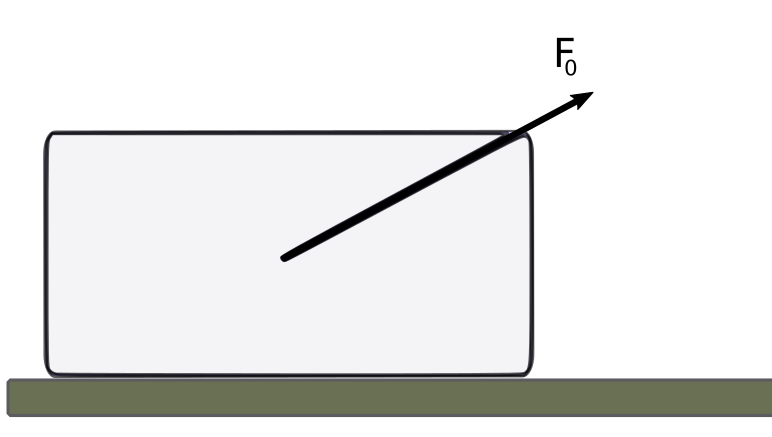
\includegraphics[scale=0.29]{Dinamika_materijalne_tocke/blok_Zadatak_4_1.png}
  \end{center}
  %\caption{Fish}
\end{figure}

%\vspace{0.2cm}
\noindent
{\color{boja} \rule{\linewidth}{0.3mm} }


$$ \vec{F}_R=\sum_i \vec{F}_i=m\vec{a}$$
$$\vec{F}_0+\vec{G}+\vec{R}+\vec{F}_{tr}=m\vec{a} $$
Radimo projekcije na $y$ i $z$ os
$$ \textbf{y:}\ \ \vec{F}_0\cdot\vec{j}+\vec{G}\cdot\vec{j}+\vec{R}\cdot\vec{j} + \vec{F}_{tr}\cdot\vec{j}= m\vec{a}\cdot\vec{j}\ \ \ \ \  /\cdot\vec{j} $$
$$ |\vec{F}_0||\vec{j}|\cos\alpha  + |\vec{G}||\vec{j}|\cos \frac{\pi}{2}  +  |\vec{R}||\vec{j}|\cos \frac{\pi}{2} +  |\vec{F}_{tr}||\vec{j}|\cos\pi
= m|\vec{a}||\vec{j}|\cos0 $$
\begin{equation}
 F_0\cos\alpha+ 0 +0 -F_{tr}=ma 
 \label{zadata_4_1_1}
\end{equation}
 


$$  \textbf{z:}\ \ \vec{F}_0\cdot\vec{k} +  \vec{G}\cdot\vec{k}  + \vec{R}\cdot\vec{k} + \vec{F}_{tr}\cdot\vec{k} = m \vec{a}\cdot\vec{k} \ \ \ \ \  /\cdot\vec{k} $$
$$   |\vec{F}_0||\vec{k}|\cos(\frac{\pi}{2}-\alpha) +|\vec{G}||\vec{k}|\cos\pi +  |\vec{R}||\vec{k}|\cos0 + 
|\vec{F}_{tr}||\vec{k}|\cos\frac{\pi}{2}=m|\vec{a}||\vec{k}|\cos\frac{\pi}{2} $$
\begin{equation}
F_0\sin\alpha-G + R =0
\label{zadata_4_1_2}
\end{equation}
Iz gornjeg izraza možemo izraziti silu reakcije podloge
$R=mg-F_0\sin\alpha$, gdje smo za silu težu ($G$) zapisali kao masa ($m$) puta ubrzanje sile teže ($g$). 

Sila trenja koja nam se javlja u izrazu \ref{zadata_4_1_1} možemo zapisati kao umonožak 
faktura kinetičkoga trenja i sili pritiska na podlogu, a sila pritiska na podlugu je jednaka težini tijela koja je po iznosu jednaka sili reakcije 
podloge tako pišemo:
$F_{tr}=\mu_k F_{\bot}=\mu_k T=\mu_k R$. 
Silu reakcije podloge možemo zamjeniti izrazom koji smo dobili iz jednadžbe \ref{zadata_4_1_2} i dobivamo konačni izraz:
$$
F_0\cos\alpha-\mu_k(mg-F_0\sin\alpha)=ma
$$
$$ a=\frac{F_0}{m}\left(\cos\alpha + \mu_k\sin\alpha\right) -\mu_k g $$

$$a = \frac{18N}{3kg}\left(\cos28^\circ + 0,4\sin28^\circ  \right) -0,4\cdot 9,81ms^{-2} =2,5\ ms^{-2} $$






\vspace{0.8cm} 



\noindent 
\textbf{\stepcounter{zadatak}
\thecjelina.\thezadatak.}
Vanjska sila iznosa $F_0=50\ N$ djeluje na blok A mase $m_A= 5\ kg$ koji vuče blok B mase $m_B= 3\ kg$ (vidjeti skicu). 
\begin{enumerate}[label=\alph*)]
 \item Izračunajte iznos sile kojom blokovi djeluju jedan na drugoga ako pretpostavimo da nema trenja.
 \item Izračunajte iznos sile kojom blokovi djeluju jedan na drugoga kada je koeficijent kinetičkog trenja između blokova i podloge $\mu_k =0,3$.
\end{enumerate}


\begin{figure}[h]%{r}{0.7\textwidth} % Inline image example
  \begin{center}
    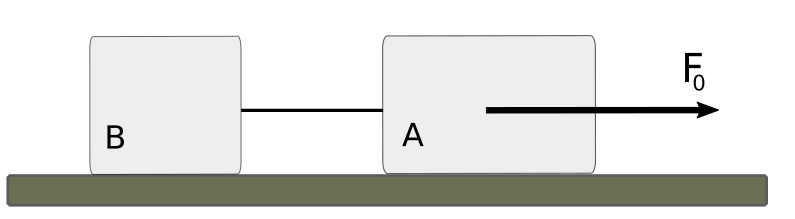
\includegraphics[scale=0.40]{Dinamika_materijalne_tocke/blok_Zadatak_4_2.png}
  \end{center}
  %\caption{Fish}
\end{figure}


\noindent
{\color{boja} \rule{\linewidth}{0.3mm} }

Iznos sile kojom blok A djeluje na blok B jednaka je iznosu sile kojom blok B djeluje na blok A 

$T=|\vec{T}_{AB}|=|\vec{T}_{BA}|$.

\begin{enumerate}[label=\alph*)]
  \item Zapišemo sve sile koje djeluju na  $$\textbf{blok B:}\ \ \ \vec{T}_{AB} + \vec{G}_B+\vec{R}_B=m_B\vec{a}\ \ \ \ \  /\cdot\vec{j}/\cdot\vec{k}$$
  $$\textbf{blok A:}\ \ \ \vec{F}_0+ \vec{T}_{BA} + \vec{G}_A+\vec{R}_A=m_A\vec{a} \ \ \ \ \  /\cdot\vec{j}/\cdot\vec{k} $$
  
  Radimo projekciju sila za blok B na os $y$ i $z$ 
  $$ \textbf{B,z:} \ \ \ 0 - G_B+R_B=0   \ \ \Rightarrow \ \  R_B=G_B$$
   $$\textbf{B,y:}\ \ \ T_{AB}+0+0=m_Ba \ \ \Rightarrow \ \ T=m_B a $$
  Isto radimo za blok A:
  $$ \textbf{A,z:}\ \ \ 0+0+G_A+R_A=0 \ \ \Rightarrow \ \  R_A=G_A  $$
   $$ \textbf{A,y:}\ \ \ F_0-T_{BA}+ 0+ 0=m_A a \ \ \Rightarrow \ \   F_0-T=m_Aa $$
 U poslijednji izraz možemo zamjeniti napetost niti $T$ sa izrazom iz $\textbf{B,y}$ 
 $$ F_0-m_B a=m_Aa $$
   $$ m_A a + m_B a =F_0$$
   $$ a= \frac{F_0}{m_A+m_B}= \frac{50N}{5kg+3kg}=6,25\ ms^{-2}$$
$$ T=m_B a=3kg\cdot 6,25ms^{-2}=18,75\ N $$   
\item
Zapišemo sve sile koje djeluju na $$\textbf{blok A:}\ \ \ \vec{F}_0+ \vec{T}_{BA} + \vec{G}_A+\vec{R}_A + \vec{F}_{tr,A}=m_A\vec{a}  \ \ \ \ \  /\cdot\vec{j}/\cdot\vec{k}$$
$$\textbf{blok B:}\ \ \ \vec{T}_{AB} + \vec{G}_B+\vec{R}_B+\vec{F}_{tr,B}=m_B\vec{a}\ \ \ \ \  /\cdot\vec{j}/\cdot\vec{k}$$
 Radimo projekciju sila za blok A na os $y$ i $z$ 
  $$ \textbf{A,y:}\ \ \ F_0-T_{BA}+ 0+ 0-F_{tr,A}=m_A a \ \ \Rightarrow \ \   F_0-T-\mu_kR_A=m_Aa $$
 $$ \textbf{A,z:}\ \ \ 0+0+G_A+R_A+0=0 \ \ \Rightarrow \ \  R_A=G_A  $$
Dobivamo $F_0-T-\mu_kG_A=m_Aa $. Isto radimo za blok B:
$$\textbf{B,y:}\ \ \ T_{AB}+0+0-F_{tr,B}=m_Ba \ \ \Rightarrow \ \ T-\mu_kR_B=m_B a $$
$$ \textbf{B,z:} \ \ \ 0 - G_B+R_B=0   \ \ \Rightarrow \ \  R_B=G_B$$
Dobivamo $T=m_Ba+\mu_kG_B$.
$$F_0 -m_Ba-\mu_km_Bg -\mu_km_Ag=m_Aa$$
Posložimo i izrazimo ubrzanje
 $$F_0-\mu_k(m_A+m_B)g=(m_A+m_B)a  $$
$$a=\frac{F_0}{m_A+m_B} -\mu_kg $$ 
$$ a=\frac{50N}{5kg+3kg} -0,3\cdot9,81ms^{-2}=3,307\ ms^{-2}$$

Još moramo izračunati napetost niti
$$ T= m_B(a+\mu_kg) $$ Ubrzanje možemo zamjeniti s dobivenim izrazom
$$ T= m_B(\frac{F_0}{m_A+m_B} -\mu_kg+\mu_kg)=\frac{m_BF_0}{m_A+m_B} $$
$$T=18,75\ N $$
   \end{enumerate}
  

\vspace{0.8cm}





\noindent 
\textbf{\stepcounter{zadatak}
\thecjelina.\thezadatak.}
Vanjska sila iznosa $F_0=42\ N$ djeluje pod kutem od $\vartheta = 30^\circ$ prema horizontali na blok $A$ mase $m_A=5 \ kg$ koji gura blok 
$B$ mase $m_B=2\ kg$ (vidjeti skicu). Izračunajte iznos ubrzanja blokova A i B kada je kinetičko trenje između blokova i podloge $\mu _k=0,3$.

\begin{figure}[h]%{r}{0.7\textwidth} % Inline image example
  \begin{center}
    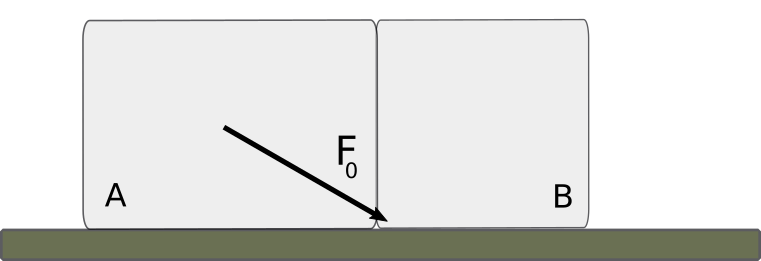
\includegraphics[scale=0.40]{Dinamika_materijalne_tocke/blok_Zadatak_4_3.png}
  \end{center}
  %\caption{Fish}
\end{figure}


\noindent
{\color{boja} \rule{\linewidth}{0.3mm} }



Iznos sile kojom blok A djeluje na blok B jednaka je iznosu sile kojom blok B djeluje na blok A 

$|\vec{F}_{AB}|=|\vec{F}_{BA}|$.

Zapisujemo sve sile na tijelo A
$$ \textbf{A:}\ \ \ \vec{F}_0+\vec{G}_A+\vec{R}_A + \vec{F}_{tr,A}+\vec{F}_{BA}=m_A\vec{a} \ \ \ \ \  /\cdot\vec{k}/\cdot\vec{j}$$
i radimo projekcije na os $z$ i $y$.
$$  \textbf{A,z:}\ \ F_0\cos(\frac{\pi}{2}+\vartheta)-m_Ag+R_A+0+0=0  $$
Funkciju $\cos(\frac{\pi}{2}+\vartheta)$ možemo raspisati preko funkcije zbroja
$$\cos(\frac{\pi}{2}+\vartheta)=\cos\frac{\pi}{2}\cos\vartheta-\sin\frac{\pi}{2}\sin\vartheta=-\sin\vartheta $$
$$-F_0\sin\vartheta-m_ag+R_A=0\ \ \Rightarrow\ \ R_A=m_Ag+F_0\sin\vartheta $$
Što ćemo ursti u izraz za $y$ os.
$$  \textbf{A,y:}\ \ F_0\cos\vartheta+0 +0 -F_{tr,A}- F_{BA}=m_Aa   $$
$$ F_0\cos\vartheta -\mu_kR_A- F_{BA}=m_Aa  $$
\begin{equation}
  F_0\cos\vartheta -\mu_k(m_Ag+F_0\sin\vartheta)- F_{BA}=m_Aa
  \label{zadata_4_3_1}
\end{equation}

Zapisujemo sve sile na tijelo B
$$ \textbf{B:}\ \ \ \vec{G}_B+\vec{R}_B + \vec{F}_{tr,B}+\vec{F}_{AB}=m_B\vec{a} \ \ \ \ \  /\cdot\vec{k}/\cdot\vec{j}$$
i radimo projekcije na os $z$ i $y$.
$$  \textbf{B,z:}\ \ -m_Bg+R_B+0+0=0  \ \ \Rightarrow\ \ R_B=m_Bg $$
$$  \textbf{B,y:}\ \ 0+0-F_{tr,B}+F_{AB}=m_Ba  \ \ \Rightarrow\ \ F_{AB}=m_Ba+\mu_kR_B$$
Spajanjem posljednja dva izraza dobivamo:
\begin{equation}
 F_{AB}=m_Ba+\mu_km_Bg.
  \label{zadata_4_3_2}
\end{equation}
U izraz \ref{zadata_4_3_1} umjesto $F_{BA}$ uvrstimo \ref{zadata_4_3_2} dobivamo:
$$  F_0\cos\vartheta -\mu_k(m_Ag+F_0\sin\vartheta)- m_Ba-\mu_km_Bg=m_Aa. $$
$$ a(m_A+m_B)= F_0\cos\vartheta -\mu_k\left[(m_A+ m_B)g+F_0\sin\vartheta\right]$$
$$ a= \frac{F_0\cos\vartheta -\mu_k\left[(m_A+ m_B)g+F_0\sin\vartheta\right]}{m_A+m_B}$$
$$ a= \frac{42N\cos30^\circ -0,3\left[(5kg+2kg)9,81ms^{-2}+42N\sin30^\circ\right]}{5kg+2kg}= 1,353\ ms^{-2}$$










\stepcounter{cjelina} 
\setcounter{zadatak}{0}




\noindent 
\textbf{\stepcounter{zadatak}
\thecjelina.\thezadatak.}
Tijelo klizi po kosini nagiba $\alpha=35^\circ$. Koeficijent kinetičkog trenja između tijela i kosine je $\mu_k=0,58$.
Izračunajete iznos ubrzanja tijela.


%\vspace{0.2cm}
\noindent
{\color{boja} \rule{\linewidth}{0.3mm} }


$$ \vec{F}_R=\sum_i \vec{F}_i=m\vec{a}$$
$$\vec{F}_0+\vec{G}+\vec{R}+\vec{F}_{tr}=m\vec{a} $$
Silu teže možemo rastaviti na dvije komponente okomito na kosinu 
$\vec{G}_{\bot}=G\cos\alpha(-\vec{k}) $ i paralelno $\vec{G}_{||}=G\sin\alpha\vec{j} $

$$ G\sin\alpha\vec{j}-G\cos\alpha\vec{k}+ R\vec{k}-F_{tr}\vec{j}= ma\vec{j}\ \ \ \ \  /\cdot\vec{j}/\cdot\vec{k}$$
Radimo projekcije na $y$ i $z$ os
$$ G\sin\alpha-0+0-F_{tr}=ma\ \ \ \Rightarrow\ \ \  G\sin\alpha-\mu_kR=ma  $$
$$ 0-G\cos\alpha+R-0=0\ \ \ \Rightarrow\ \ \  R=G\cos\alpha $$


$$G\sin\alpha-\mu_kG\cos\alpha=ma  $$
$$mg\sin\alpha-\mu_kmg\cos\alpha=ma  $$
$$a=g(\sin\alpha-\mu_k\cos\alpha)  $$
$$a=9,81ms^{-2}(\sin35^\circ-0,58\cos35^\circ)= 0,966\ ms^{-2} $$

\vspace{0.8cm} 




\noindent 
\textbf{\stepcounter{zadatak}
\thecjelina.\thezadatak.}
Na slici dolje je sustav od dva utega mase $m_A=10\ kg$ i $m_B=5\ kg$. Uteg B povezan je tankom nerastezljivom niti s utegom A. 
Kosina na kojoj se nalazi uteg A nagnuta je pod kutom $\alpha=30^\circ$, a koeficijent kinetičkog trenja između kosine i utega A iznosi $\mu_k=0,2$.
\begin{enumerate}[label=\alph*)]
 \item Skicirajte problem i označite sve sile i smjer gibanja (vektor ubrzanja) cijelog sustava.
 \item Izračunajte iznos ubrzanja cijelog sustava.
 \item Izračunajte iznos sile napetosti niti.
\end{enumerate}
\begin{figure}[h]%{r}{0.7\textwidth} % Inline image example
  \begin{center}
    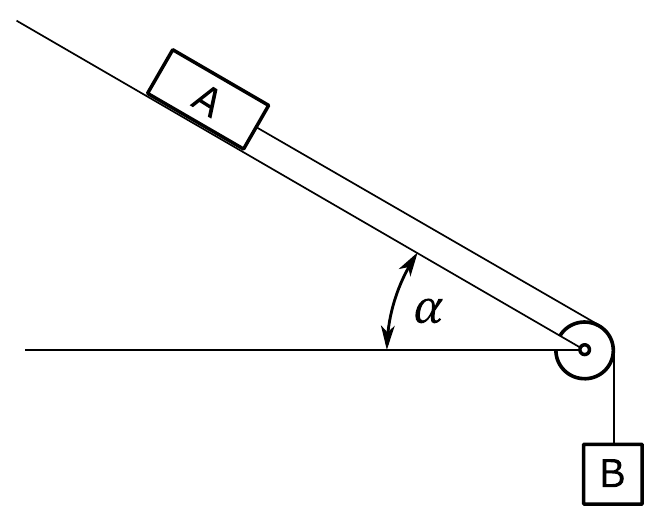
\includegraphics[scale=0.40]{Dinamika_materijalne_tocke/kosina_5_2.png}
  \end{center}
  %\caption{Fish}
\end{figure}

\noindent
{\color{boja} \rule{\linewidth}{0.3mm} }


\begin{enumerate}[label=\alph*)]
\item Na tijelo A djeluju sila teže ($\vec{G}_A$) prema dolje koju rastavljamo na dvije komponente:
silu okomitu na kosinu ($ \vec{G}_{A,\bot}$) i silu usporednu s kosinom prema dolje ($\vec{G}_{A,||} $), zatim djeluje sila 
trenja ($\vec{F}_{tr,A} $), sila reakcije podloge $\vec{R}_A$ i sila kojom uteg B vuče uteg A (sila napetosti niti $\vec{T}_{BA} $).  
Na uteg B djeluju samo dvije sile, sila teža prema dolje ($\vec{G}_B$) i napetost niti prema gore ($\vec{T}_{AB}$).

Sila napetosti niti kojom djeluje uteg A na uteg B jednaka je po iznosu sili napetosti kojom uteg B djeluje na uteg A stoga pišemo
$$ |\vec{T}_{AB}|=|\vec{T}_{BA}|=T. $$ 
\item 
Za uteg B možemo pisati
$$\vec{G}_B+\vec{T}_{AB}=m_B\vec{a},$$
\begin{equation}
 G_B-T=m_Ba   \ \ \Rightarrow \ \  T=m_B(g-a).  
 \label{zadatak_5_2_1}
\end{equation}
Zapisujemo sve sile koje djeluju na uteg A
$$ \vec{G}_{A,||}+\vec{G}_{A,\bot}+\vec{R}_A+\vec{F}_{tr,A} + \vec{T}_{BA}=m_A\vec{a}.  $$
Radimo projekciju sila na smjer gibanja
$$ G_{A,||} -F_{tr,A}+T=m_A a  $$
$$ m_Ag\sin\alpha-\mu_k m_Ag\cos\alpha +T = m_Aa $$
Napetost niti možemo zamjeniti izrazom \ref{zadatak_5_2_1} i dobivamo
$$ m_Ag\sin\alpha-\mu_k m_Ag\cos\alpha +m_Bg-m_Ba = m_Aa. $$ 
Nakom sređivanja dobivamo konačni izraz
$$ (m_A\sin\alpha-\mu_k m_A\cos\alpha +m_B)g =( m_A+m_B)a $$
$$a=\frac{m_A(\sin\alpha-\mu_k \cos\alpha) +m_B}{ m_A+m_B}\ g. $$
Uvrstimo zadane vrijednosti
$$a=\frac{10\ kg(\sin30^\circ-0,2\cos30^\circ)}{10\ kg+5\ kg}\ 9,81\ ms^{-2}=5,41 \ ms^{-2}$$

 \item Kako bismo dobili iznos sile napetosti niti uvrštavamo dobivenu akceleraciju u izrac \ref{zadatak_5_2_1}
 $$ T=5\ kg(9,81 \ ms^{-2}- 5,41 \ ms^{-2})=22\ N $$
 
 
\end{enumerate}



\vspace{0.8cm}




\noindent 
\textbf{\stepcounter{zadatak}
\thecjelina.\thezadatak.}
Koeficijent kinetičkog trena između blokova i podloge je $\mu_k=0,2$, a dimenzije i mase su: $a=5\ m$, $b=3\ m$, $v=4\ m$, $m_A=10\ kg$ i $m_B=15\ kg$.
Koliki je iznos ubrzanja blokova prikazanih na slici?
\begin{figure}[h]%{r}{0.7\textwidth} % Inline image example
  \begin{center}
    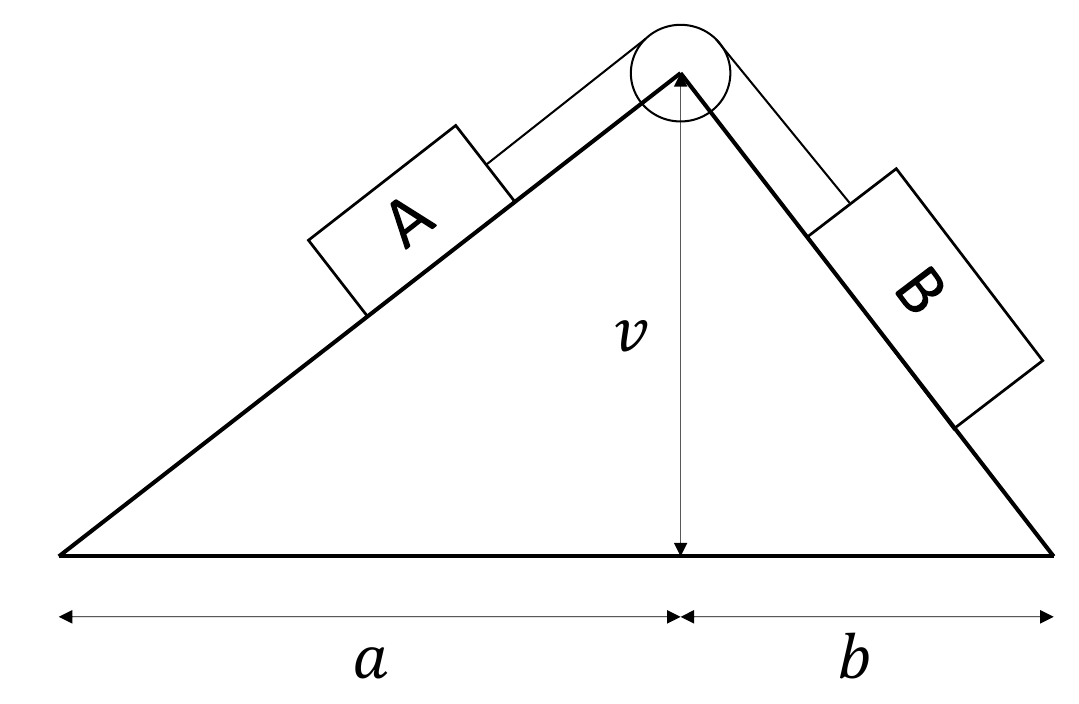
\includegraphics[scale=0.30]{Dinamika_materijalne_tocke/kosina_5_3.png}
  \end{center}
  %\caption{Fish}
\end{figure}


\noindent
{\color{boja} \rule{\linewidth}{0.3mm} }

Sila napetosti niti kojom djeluje blok A na blok B jednaka je po iznosu sili napetosti kojom uteg B 
djeluje na uteg A stoga pišemo
$$ |\vec{T}_{AB}|=|\vec{T}_{BA}|=T. $$ 
Kako bismo mogli rastaviti sile moramo izračunati kuteve $\alpha$ i $\beta$
$$\tan\alpha=\frac{v}{a}   \ \ \Rightarrow \ \  \alpha=\arctan\frac{4m}{5m}=38,66^\circ, $$
$$\tan\beta=\frac{v}{b}   \ \ \Rightarrow \ \  \beta=\arctan\frac{4m}{3m}=53,13^\circ .$$
Zapisujemo sve sile koje djeluju na blok A i množimo skalarno s $\cdot\vec{j}$ 
$$\vec{G}_{A,||} + \vec{G}_{A,\bot} + \vec{R}_A + \vec{F}_{tr,A} + \vec{T}_{BA}=m_A \vec{a}  \ \ \ \  /\cdot\vec{j}   $$
Dobivamo sile u usporedne s lijevim nagibom kosine
$$ -m_Ag\sin\alpha - \mu_km_Ag\cos\alpha + T =m_Aa. $$
Izrazimo napetosti niti
\begin{equation}
 T= m_Ag\sin\alpha + \mu_km_Ag\cos\alpha + m_Aa. 
 \label{zadatak_5_3_1}
\end{equation}
 
Isto radimo za blok B
$$\vec{G}_{B,||} + \vec{G}_{B,\bot} + \vec{R}_B + \vec{F}_{tr,B} + \vec{T}_{AB}=m_B \vec{a}  \ \ \ \  /\cdot\vec{j}   $$
\begin{equation}
 m_Bg \sin\beta - \mu_km_Bg\cos\beta - T =m_Ba
 \label{zadatak_5_3_2}
\end{equation} 
Uvrštavamo izraz \ref{zadatak_5_3_1} za napetost niti u izraz \ref{zadatak_5_3_2}
$$ m_Bg \sin\beta - \mu_km_Bg\cos\beta - m_Ag\sin\alpha - \mu_km_Ag\cos\alpha - m_Aa =m_Ba.$$
Sređujemo izraze:
$$ g\left[ m_B(\sin\beta - \mu_k\cos\beta ) - m_A (\sin\alpha + \mu_k\cos\alpha) \right] =(m_A + m_B)a$$
$$ a = \frac{m_B(\sin\beta - \mu_k\cos\beta ) - m_A (\sin\alpha + \mu_k\cos\alpha)}{m_A + m_B}\ g$$
$$ a = \frac{15kg(\sin53,13^\circ - 0,2\cos53,13^\circ) - 10kg(\sin38,66^\circ + 0,2 \cos38,66^\circ )}
{10kg+15kg}\ 9,81 \ ms^{-2} $$

$$a = 0,94  \ ms^{-2}  $$








\vspace{1cm}


\noindent 
\textbf{\stepcounter{zadatak}
\thecjelina.\thezadatak.}
Na blok mase $m = 2\ kg$ djelujemo silom $F = 25,0\ N$
usporedno s nagibom kosine (kao na slici). Ako je kosina
nagiba $\alpha = 39^\circ$, a koeficijent kineti\v{c}kog trenja između
bloka i podloge $\mu_k = 0,25$ koliko je ubrzanje bloka?
\begin{figure}[h]%{r}{0.3\textwidth} % Inline image example
  \begin{center}
    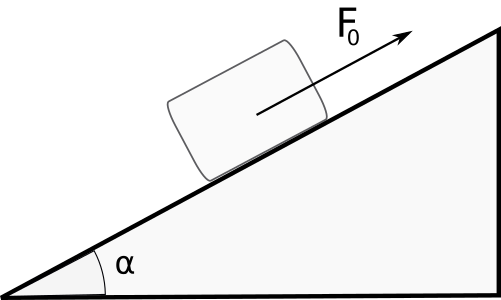
\includegraphics[width=0.3\textwidth]{Dinamika_materijalne_tocke/kosina.png}
  \end{center}
  %\caption{Fish}
\end{figure}


\noindent
{\color{boja} \rule{\linewidth}{0.3mm} }


$a=4,420\ ms^{-2}$


\vspace{1.5cm}


\noindent 
\textbf{\stepcounter{zadatak}
\thecjelina.\thezadatak.}
Dva bloka mase $m_A = 10\ kg$ i $m_B = 8\ kg$ spojena su nerastezljivim užetom i položena na kosinu
nagiba $\alpha = 33^\circ$ kao na slici. Ako je koeficijent kineti\v{c}kog trenja izme\dj{}u bloka A i kosine je 
$\mu_{kA} = 0,4$,
a između bloka B i kosine je $\mu_{kB} = 0,2$ izra\v{c}unajte iznos ubrzanja cijelog sustava.
\begin{figure}[h]%{r}{0.35\textwidth} % Inline image example
  \begin{center}
    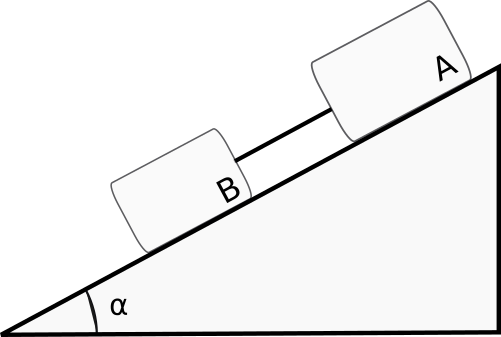
\includegraphics[width=0.3\textwidth]{Dinamika_materijalne_tocke/kosina2.png}
  \end{center}
  %\caption{Fish}
\end{figure}


\noindent
{\color{boja} \rule{\linewidth}{0.3mm} }


$a=2,783\ ms^{-2}$



\vspace{1.5cm}


\noindent 
\textbf{\stepcounter{zadatak}
\thecjelina.\thezadatak.}
Blok $m_A = 7\ kg$ položen je na ravni dio klina, a blok $m_B = 15\ kg$ polo\v{z}en je na kosi dio
klina nagiba $\alpha = 37^\circ$.
\begin{enumerate}[label=\alph*)]
 \item Izra\v{c}unajte iznos akceleracije sustava ako pretpostavimo da nema trenja.
 \item Izra\v{c}unajte iznos akceleracije sustava kada je koeficijent kineti\v{c}kog trenja izme\dj{}u
blokova i podloge μk = 0,1.
\end{enumerate}
\begin{figure}[h]%{r}{0.35\textwidth} % Inline image example
  \begin{center}
    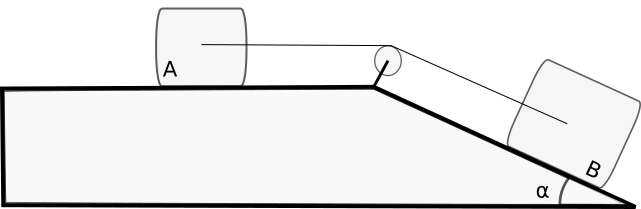
\includegraphics[width=0.5\textwidth]{Dinamika_materijalne_tocke/stol_i_kosina.png}
  \end{center}
  %\caption{Fish}
\end{figure}


\noindent
{\color{boja} \rule{\linewidth}{0.3mm} }

\begin{enumerate}[label=\alph*)]
 \item $a=4,025\ ms^{-2}$
\item $a=3,803\ ms^{-2}$
\end{enumerate}


\newpage
\chapter{ZAKONI OČUVANJA}
\stepcounter{cjelina} 
\setcounter{zadatak}{0}




\noindent 
\textbf{\stepcounter{zadatak}
\thecjelina.\thezadatak.}
Materijalna točka pomaknuta je u $xy-$ravnini iz točke A čiji je vektor položaja $\vec{r}_A=\vec{i}+2\vec{j}\ \left[m\right]$ u točku B kojoj je vektor položaja 
$\vec{r}_B=2\vec{i}-3\vec{j}\ \left[m\right]$. Tijekom pomaka na nju je djelovala stalna sila $\vec{F}=3\vec{i}+4\vec{j}\ \left[N\right]$.
Izračunajte rad sile $\vec{F}$.


%\vspace{0.2cm}
\noindent
{\color{boja} \rule{\linewidth}{0.3mm} }


$$W_{F,AB}=\int_{r_A}^{r_B} \vec{F}\cdot d\vec{r} $$

$$\vec{F}=konst.   \ \ \Rightarrow \ \    W_{F,AB}=\vec{F}\cdot\Delta\vec{r} $$
$$\Delta\vec{r}\equiv\vec{r}_B-\vec{r}_A $$
$$\Delta\vec{r}=(2\vec{i} - 3\vec{j}) - (\vec{i} + 2\vec{j} )=\vec{i} - 5\vec{j} $$
$$ W_{F,AB}= (3\vec{i} + 4\vec{j})\cdot(\vec{i} - 5\vec{j}) = -17\ J $$


\vspace{0.8cm} 



\noindent 
\textbf{\stepcounter{zadatak}
\thecjelina.\thezadatak.}
Tijelo počinje klizati iz stanja mirovanja na visini od $0,8$ metara na vrhu kosine. Kolika je brzina tijela na dnu kosine ako je nagib kosine $30^\circ$,
koeficijent kinetičkog trenja $0,43$?


\noindent
{\color{boja} \rule{\linewidth}{0.3mm} }


Pišemo zakon očuvanja energije
$$ E_k(B) + E_{p,G}(B)  = E_k(A) + E_{p,G}(A) + W_{AB}$$
$$ \frac{1}{2}mv^2 + 0 = 0 + mgH + \vec{F}_{tr}\cdot\Delta\vec{r}  $$
Ostalo je za izračunati rad sile trenja
$$\vec{F}_{tr}\cdot\Delta\vec{r}=|\vec{F}_{tr}||\Delta\vec{r}|\cos \sphericalangle (\vec{F}_{tr},\Delta\vec{r})
=F_{tr}\Delta r\cos(\pi)$$
Pomak tijela $\Delta r$ možemo izaraziti iz visine kosine i kuta $\Delta r=H/\sin\vartheta$. Potrebno je 
još zapisati silu trenja koja ovisi o kinematičkom koeficijentu trenja i sili kojom tijelo pritišće podlogu
$F_{tr} = \mu_kmg\cos\vartheta $.
$$\vec{F}_{tr}\cdot\Delta\vec{r}= - \mu_kmg\cos\vartheta\frac{H}{\sin\vartheta}= - \mu_k mgH\cot\vartheta$$
Vraćamo se u zakon očuvanja energije
$$ \frac{1}{2}mv^2 = mgH - \mu_k mgH\cot\vartheta  $$
$$ v=\sqrt{2gH(1 - \mu_k\cot\vartheta)}$$
$$ v = \sqrt{2 \cdot 9,81 \ ms^{-2} \cdot 0,8 \ m (1-0,43\cdot\cot30^\circ)}=2,0 \ ms^{-1} $$



\vspace{0.8cm}




\noindent 
\textbf{\stepcounter{zadatak}
\thecjelina.\thezadatak.}
Konstanta opruge koja se koristi za ispucavanje kuglice flipera mase $80$ grama je $138\ Nm^{-1}$.
Koliko centrimetara treba povući ručicu flipera (tj. stisnuti oprugu) da bi se kuglica ispalila brzinom iznosa $5 ms^{-1}$?


\noindent
{\color{boja} \rule{\linewidth}{0.3mm} }


Pišemo zakon očuvanja energije
$$ E_k(B) + E_{p,el}(B)  = E_k(A) + E_{p,el}(A) + W_{AB}$$
$$ 0 + \frac{1}{2}mv^2= \frac{1}{2}K\Delta x^2 + 0 + 0$$
$$ \frac{1}{2}mv^2= \frac{1}{2}K\Delta x^2$$
$$ \Delta x=v\sqrt{\frac{m}{K}} $$

$$ \Delta x = 5 ms^{-1} \sqrt{\frac{0,08 kg}{138Nm^{-1}}}=0,12\ m $$


\vspace{1cm}

\noindent 
\textbf{\stepcounter{zadatak}
\thecjelina.\thezadatak.}
S vrha strme ceste duga\v{c}ke $100\ m$, visinske razlike $20\ m$, spu\v{s}taju se saonice mase $5\ kg$.
Izra\v{c}unajte iznos sile trenja koja se javlja pri spu\v{s}tanju niz brijeg ako saonice na dnu brijega
imaju brzinu $16\ ms^{-1}$. Po\v{c}etna brzina saonica je nula.


\noindent
{\color{boja} \rule{\linewidth}{0.3mm} }


$F_{tr}=3,41\ N$


\vspace{1cm}

\noindent 
\textbf{\stepcounter{zadatak}
\thecjelina.\thezadatak.}
Iz stanja mirovanja na visini $h = 0,8\ m$ na vrhu kosine tijelo po\v{c}inje kliziti niz kosinu te
kad do\dj{}e do dna kosine nastavi još \v{c}etiri metra kliziti horizontalno prije nego se zaustavi.
Koeficijent kineti\v{c}kog trenja $\mu_k$ izme\dj{}u tijela i podloge je isti kad tijelo klizi niz kosinu i
horizontalno. Koliki je $\mu_k$ ako je nagib kosine $\vartheta = 20^\circ$?


\noindent
{\color{boja} \rule{\linewidth}{0.3mm} }


$\mu_k=0,129$


\vspace{1cm}

\noindent 
\textbf{\stepcounter{zadatak}
\thecjelina.\thezadatak.}
Materijalna to\v{c}ka mase $m = 0,5\ kg$ giba se u $xy$-ravnini iz točke A čiji je vektor položaja
$\vec{r}_A = 11\vec{i} - 9\vec{j}\ [m]$ u točku B kojoj je vektor položaja $\vec{r}_B= -7\vec{i} + 12\vec{j}\ [m]$. Na putanji do to\v{c}ke B na nju djeluje rezultantna sila $\vec{F}_R = -3\vec{i} + \vec{j}\ [N]$. Izračunajte 
kolika \'{c}e biti kineti\v{c}ka energija u to\v{c}ki B ako je brzina u to\v{c}ki A bila $\vec{v}_A = 3\vec{i} + 4\vec{j}\ [ms^{ -1} ]$?


\noindent
{\color{boja} \rule{\linewidth}{0.3mm} }


$E_k (B) = 81,25\ J$



\vspace{1cm}

\noindent 
\textbf{\stepcounter{zadatak}
\thecjelina.\thezadatak.}
Dječak s mosta visokog $5\ m$ iznad rijeke baci loptu vertikalno u zrak brzinom $11\ kmh^{-1}$.
Na kojoj visini iznad rijeke bi potencijalna energija bila jednaka kinetičkoj, kad bi mogli
zanemariti otpor zraka?



\noindent
{\color{boja} \rule{\linewidth}{0.3mm} }


$h= 2,738\ m$


\vspace{1cm}

\noindent 
\textbf{\stepcounter{zadatak}
\thecjelina.\thezadatak.}
Tijelo mase $10\ g$ nalazi se na vertikalno postavljenoj opruzi u stanju ravnoteže. Konstanta
opruge je $100\ Nm^{ −1}$ pa se deformacija opruge zbog težine tijela (oko $1\ mm$) može slobodno
zanemariti. Vanjska sila oprugu stisne za $5\ cm$. Taj novi položaj tijela uzima se kao početna
visina $h_1 = 0$. Do koje maksimalne visine $h_2$ ovako stisnuta opruga može izbaciti tijelo? Otpor zraka se zanemaruje.


\noindent
{\color{boja} \rule{\linewidth}{0.3mm} }


$h_2= 1,274$




\stepcounter{cjelina} 
\setcounter{zadatak}{0}



\noindent 
\textbf{\stepcounter{zadatak}
\thecjelina.\thezadatak.}
Automobil mase $m=2000\ kg$ giba se uz kosinu nagiba $\vartheta=15^\circ $ stalnom brzinom iznosa $60\ kmh^{-1}$.
Ukupna sila otpora (trenje kotrljanja i otpor zraka) iznosi $| \vec{F}_{otp}|=2000\ N $, a visina kosine je 
$h=60\ m$. Izračunajte: 
\begin{enumerate}[label=\alph*)]
 \item pogonsku silu automobila;
 \item rad pogonske sile od početka do kraja kosine;
 \item snagu automobila.
\end{enumerate}

%\vspace{0.2cm}
\noindent
{\color{boja} \rule{\linewidth}{0.3mm} }


\begin{enumerate}[label=\alph*)]
 \item Ako je brzina stalna tada je rezultantna sila na automobil jednaka je nuli; 
$\vec{v}=konstanta    \ \ \Rightarrow \ \ \vec{F}_R=\vec{0}.$

$$ \vec{F} + \vec{F}_{otp} + \vec{G}_{||} + \vec{G}_{\bot} + \vec{R} = \vec{0} \ \ \ \  /\cdot\vec{j} $$
$$ F - F_{otp} - mg\sin\vartheta = 0$$
$$ F = F_{otp} + mg\sin\vartheta  $$
$$ F = 2000N + 2000kg\ 9,81ms^{-2}\ \sin15^\circ = 7078,03\ N $$
 \item  $$ W=\vec{F}\Delta \vec{r}=F\Delta r\cos 0^\circ $$
 Pomak automobila možemo izraziti preko visine kosine i kuta
 $$ W = F\frac{h}{\sin\vartheta} = 7078,03\frac{60m}{\sin15^\circ} = 1640844\ J $$
 \item $$ P = \vec{F}\cdot\vec{v}=Fv $$
Iznos brzine automobila je $ v = 60\ kmh^{-1} = 60\frac{1000\ m}{3600\ s}=16,67\ ms^{-1}$
$$P=7078,03\ N 16,67\ ms^{-1} = 117967\ W$$
\end{enumerate}

\vspace{0.8cm} 



\noindent 
\textbf{\stepcounter{zadatak}
\thecjelina.\thezadatak.}
Ledolomac mase $6000$ tona s ugašenim motorom nalijeće brzinom $30\ kmh^{-1}$ na santu leda koja se giba brzinom $2\ kmh^{-1}$ 
u istom smjeru. Poslije sudara zajedno se kreću brzinom $5\ kmh^{-1}$. Kolika je masa sante leda?


\noindent
{\color{boja} \rule{\linewidth}{0.3mm} }

Zapisujemo zakona očuvanja količine gibanja i izražavamo masu sante leda

$$ m_1v_1 + m_2v_2=(m_1 + m_2)v'$$
$$m_2v_2 - m_2v' = m_1v' - m_1v_1 $$
$$ m_2 = \frac{v' - v_1}{v_2 - v'}m_1 $$
$$ m_2 = \frac{5\ kmh^{-1} - 30\ kmh^{-1} }{2\ kmh^{-1} - 5 \ kmh^{-1}}6000 \ t =50 000\ t $$
\vspace{0.8cm}


\noindent 
\textbf{\stepcounter{zadatak}
\thecjelina.\thezadatak.}
Klizač mase $70\ kg$ koji stoji na ledu odbacuje od sebe u horizontalnom smjeru predmet mase $3\ kg$ brzinom od $8\ ms^{-1}$.
Koliko će se klizač pomaknuti, ako je koeficijent kinetičkog trenja između leda i klizaljki $0,02$?



\noindent
{\color{boja} \rule{\linewidth}{0.3mm} }

Prije početka gibanja klizač miruje zajedno s predmetom $v'=0 $ stoga možemo izraziti
iz zakona očuvanja količine gibanja brzinu klizača na početku njegovog gibanja
$$ (m_1+m_2)v'=m_1v_1+m_2v_2  $$
$$ 0 = m_1v_1+m_2v_2  \ \ \Rightarrow \ \  v_1=-\frac{m_2}{m_1} v_2$$
Zapisujemo zakon očuvanja energije za klizača 
$$  E_k(B) + E_{p}(B)  = E_k(A) + E_{p}(A) + W_{AB}.$$ 
Budući da nema promjene visine potencijalna energija klizača je jednaka nuli, a kako na kraju svojega gibanja staje njegova kinetička energija $E_k(B)$ će također biti jednaka nuli
$$ 0 + 0 = \frac{1}{2}mv_1^2 + 0 + \vec{F}_{tr}\cdot\Delta\vec{r}$$
$$  0 = \frac{1}{2}mv_1^2 + F_{tr} \Delta r\cos\sphericalangle(\vec{F}_{tr},\Delta\vec{r})  $$ 
$$  0 = \frac{1}{2}mv_1^2 + F_{tr} \Delta r\cos\pi  $$ 
$$  \Delta r= \frac{1}{2} \frac{v_1^2}{\mu_k g} = \frac{m_2^2v_2^2}{2\mu_k m_1^2 g} $$
$$  \Delta r = \frac{(3\ kg)^2\cdot (8\ ms^{-1})^2 }{2\cdot 0,02 \cdot (70\ kg)^2 \cdot 9,81\ ms^{-2}}=0,3\ m $$





\vspace{1cm}

\noindent 
\textbf{\stepcounter{zadatak}
\thecjelina.\thezadatak.}
Kolikom se maksimalnom brzinom izraženom u kilometrima na sat može gibati automobil
mase $1400\ kg$ i snage $45\ kW$ po cesti na kojoj je koeficijent kinetičkog trenja 0,08? (Otpor
zraka se zanemaruje.)

\noindent
{\color{boja} \rule{\linewidth}{0.3mm} }

$v_{max}= 147,44\ kmh^{-1}$



\vspace{1cm}

\noindent 
\textbf{\stepcounter{zadatak}
\thecjelina.\thezadatak.}
Automobil mase $1500\ kg$ koji se gibao brzinom $45\ kmh^{-1}$ udario je u kamion mase 6 tona koji se u istom smjeru gibao 
brzinom $18 \ kmh^{-1}$. U trenutku sudara prestali su im raditi motori te su se nastavili zajedno gibati još 26 metara dok se nisu zaustavili. Koliki je bio iznos sile trenja tijekom zaustavljanja?

\noindent
{\color{boja} \rule{\linewidth}{0.3mm} }

$F_{tr}=6093,75$


\vspace{1cm}

\noindent 
\textbf{\stepcounter{zadatak}
\thecjelina.\thezadatak.}
Automobil mase $1500\ kg$ koji se gibao brzinom $45\ kmh^{-1}$ udario je u kamion mase 6 tona koji se u istom smjeru gibao 
brzinom $18 \ kmh^{-1}$. U trenutku sudara prestali su im raditi motori te su se nastavili zajedno gibati još 26 metara dok se nisu zaustavili. Koliki je bio iznos sile trenja tijekom zaustavljanja?

\noindent
{\color{boja} \rule{\linewidth}{0.3mm} }

$F_{tr}=6093,75$



\newpage
\chapter{KRUTO TIJELO}
\stepcounter{cjelina} 
\setcounter{zadatak}{0}




\noindent 
\textbf{\stepcounter{zadatak}
\thecjelina.\thezadatak.}
Kotač promjera 40 $cm$ vrti se oko nepomične osi tako da se kut zakreta mijenja u vremenu prema sljedećem izrazu:
$$
\varphi(t)=5t+3t^2+4t^4\ [rad].
$$
Izračunajte:
\begin{enumerate}[label=\alph*)]
 \item Kutnu brzinu vrtnje u trenutku $t=0,5\ s$.
 \item Obodnu brzinu ruba kotača u trenutku $t=0,5\ s$.
 \item Kutno ubrzanje u trenutku $t=0,5\ s$.
 \item Koliko okretaja napravi kotač od $t=0\ s$ do $t=0,5\ s$.
\end{enumerate}

%\vspace{0.2cm}
\noindent
{\color{boja} \rule{\linewidth}{0.3mm} }

\begin{enumerate}[label=\alph*)]
\item 

$\omega(t)=\frac{d\varphi(t)}{dt} = \frac{d}{dt}(5t+3t^2+4t^4)$

$\omega(t)=5+6t+16t^3$

$\omega(t=0,5\ s)=5+6\cdot0,5+16\cdot 0,5^3=10\ rad s^{-1}$
\item

$v(t)=\omega(t)r=(5+6t+16t^3)r$

$v(t=0,5\ s)=\omega(t=0,5)r=10\ rad s^{-1}0,2\ m=2\ ms^{-1} $

\item

$\alpha(t)=\frac{d\omega(t)}{dt}=\frac{d}{dt}(5+6t+16t^3)=6+48t^2 $

$\alpha(t=0,5\ s)=6+48\cdot 0,5^2=18\ rad s^{-2}$

\item Označimo broj okretaja s $n$

$n 2\pi= \Delta\varphi$

$n=\frac{1}{2\pi}(\varphi(0,5\ s)-\varphi(0\ s))$

$n=\frac{1}{2\pi}(5\cdot0,5+3\cdot0,5^2+4\cdot0,5^4-0)=0,557$ okretaja.

\end{enumerate}

\vspace{0.8cm} 



\noindent 
\textbf{\stepcounter{zadatak}
\thecjelina.\thezadatak.}
Homogeni aluminijski valjak polumjera 8 i visine 32 $cm$ rotira oko osi koja je paralelna s osi valjka, a prolazi kroz plašt.
Odredite kinetičku energiju rotacije ako napravi 105 okretaja u minuti. Gustoća aluminija je $2,7\ gcm^{-3}$.


\noindent
{\color{boja} \rule{\linewidth}{0.3mm} }

Kako bismo izračunali kinetičku energiju rotacije $E_k= \frac{1}{2}I\omega^2$ moramo znati moment tromosti oko osi rotacije i iznos kutne brzine. Kako bismo odredili moment tromosti koristimo teorem o paralelnim osima (Steinerov teorem):
$$ I=I_T+Md^2 $$
gdje je $I_T$ moment tromosti oko osi koja prolazi kroz centar mase i za valjak iznosi $I_T=\frac{1}{2}MR^2$, $M$ je u ovom slučaju masa valjka, a $d$ je udaljenost između osi koja prolazi centrom mase i osi rotacije. Tako da moment tromosti možemo pisati 
$$I=\frac{1}{2}MR^2+MR^2=\frac{3}{2}MR^2. $$
Masu valjka možemo izraziti preko gustoće i volumena valjka ($V=R^2\pi h$), 
$$I=\frac{3}{2}\pi\rho h  R^4 .$$
Ostalo je izračunati kutnu brzinu koja je broj okretaja u sekunti puta $2\pi$
$$\omega=\frac{105}{60\ s}2\pi\ rad=10,995\ rads^{-1}\simeq11\ rads^{-1} $$.
Sada možemo izračunati kinetičku energiju rotacije:
$$E_k= \frac{3}{4}\pi\rho h  R^4 \omega^2 =\frac{3}{4}\pi 2700\ kgm^{-3}(0,08\ m)^4 0,32\ m (11\  rads^{-1})^2
$$

$$E_k=10,0895\ J $$

\vspace{0.8cm}




\noindent 
\textbf{\stepcounter{zadatak}
\thecjelina.\thezadatak.}
Dvije homogene kugle gustoće $2700\ kgm^{-3}$ i polumjera $4\ cm$ spojene su štapom zanemarive mase i duljine $10\ cm$ (vidi skicu).
Koliki je moment susutava oko osi koja prolazi polovištem štapa? Moment tromosti kugle oko osi koja prolazi kroz središte je $I=\frac{2}{5}MR^2$.
\begin{figure}[h]%{r}{0.7\textwidth} % Inline image example
  \begin{center}
    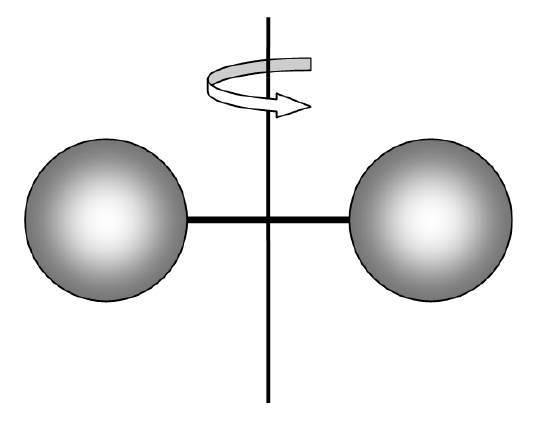
\includegraphics[scale=0.40]{Kruto_tijelo/kugle.png}
  \end{center}
  %\caption{Fish}
\end{figure}



\noindent
{\color{boja} \rule{\linewidth}{0.3mm} }


Moment tromosti sustava $I$ je zbroj momenta tromosti svake kugel, $I=2I_{kugla}$
Kako bismo odredili moment tromosti kugle koristimo teorem o paralelnim osima (Steinerov teorem):
$$
I_{kugla}= I_T+Md^2
$$

$$
I_{kugla}=\frac{2}{5}MR^2+M(\frac{L}{2}+R)^2
$$
gdje je $M$ masa jedne kugle, $R$ je njezin radijus, a $L$ je udaljenost između kugli. Udaljenost osi rotacije od centra mase kugle je $d=\frac{L}{2}+R$. Izrazimo masu pomoću gustoće i volumena kugle ($V=\frac{4}{3}R^3\pi$) i dobivamo moment tromosti jedne kugle:
$$
I_{kugle}=\frac{4}{3}\pi\rho R^3\left[\frac{2}{5}R^2 + \left(\frac{L}{2}+R \right)^2\right].
$$
Moment tromosti sustava je:
$$
I=2I_{kugle}=\frac{8}{3}\pi2700\ kgm^{-3} (0,04\ m)^3\left[\frac{2}{5}(0,04\ m)^2 + \left(\frac{0,1\ m}{2}+(0,04\ m) \right)^2\right]
$$

$$ I=0,01265\ kgm^2.$$


%\vspace{0.8cm}

\vspace{1cm}


\noindent 
\textbf{\stepcounter{zadatak}
\thecjelina.\thezadatak.}
Kotač se vrti oko nepomične osovine tako da mu se kut zakreta mijenja u vremenu
prema izrazu
$$
\varphi(t) = t e^{-0,1t} [rad].
$$
Izra\v{c}unajte:
\begin{enumerate}[label=\alph*)]
 \item Kutnu brzinu vrtnje u trenutku $t=3\ s$.
 \item Kutno ubrzanje u trenutku $t=3\ s$.
\end{enumerate}

\noindent
{\color{boja} \rule{\linewidth}{0.3mm} }


\begin{enumerate}[label=\alph*)]
\item 
$\omega(t=3\ s)=0,519\ rad/s$

\item 
$\alpha(t=3\ s)=-0,126\ rad/s^2$
\end{enumerate}




\vspace{1cm}


\noindent 
\textbf{\stepcounter{zadatak}
\thecjelina.\thezadatak.}
Koliko okretaja u minuti treba rotirati homogeni mjedeni valjak oko osi koja je paralelna s osi valjka a prolazi kroz pla\v{s}t, da bi mu kineti\v{c}ka energija rotacije bila $40\ J$? Visina valjka je $30\ cm$, a polumjer $10\ cm$. Gustoća mjedi je $8,5\ g/cm^3$.



\noindent
{\color{boja} \rule{\linewidth}{0.3mm} }

$\nu = 77,92\ okr/min $


\vspace{1cm}


\noindent 
\textbf{\stepcounter{zadatak}
\thecjelina.\thezadatak.}
Na valjak polumjera $R$ i mase $M$ koji se može rotirati oko horizontalne osi namotana je nit na koju je obje\v{s}en uteg mase
$m$ (vidi skicu). Kolika će biti kutna brzina valjka u trenutku kad uteg padne s visine $h$?
\begin{figure}[h]%{r}{0.7\textwidth} % Inline image example
  \begin{center}
    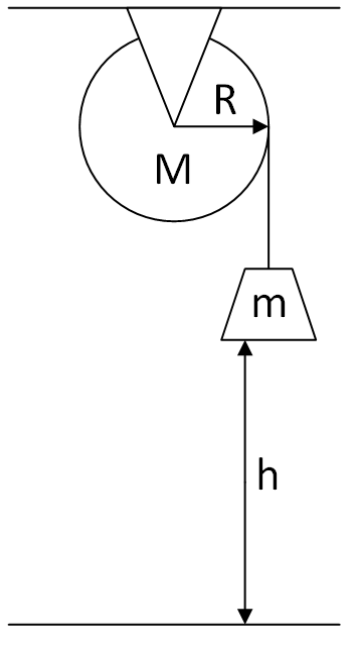
\includegraphics[scale=0.40]{Kruto_tijelo/zadatak_R901.png}
  \end{center}
  %\caption{Fish}
\end{figure}



\noindent
{\color{boja} \rule{\linewidth}{0.3mm} }

$\omega= \sqrt{\frac{4mgh}{R(2m+M)}}$






\stepcounter{cjelina} 
\setcounter{zadatak}{0}

\newpage
\chapter{GRAVITACIJA}

\textit{Kod rješavanja zadataka koristite se sljedećim numeričkim vrijednostima:
\begin{itemize}
 \item gravitacijska konstanta: $\gamma = 6,67\cdot  10^{−11}\ Nm^2kg^{−2}$
 \item masa Zemlje: $M_Z = 5,98 \cdot  10^{24}\ kg$
 \item polumjer Zemlje: $R_Z = 6,371 \cdot 10^6\ m$
 \item iznos ubrzanja slobodnog pada: $g = 9,81\ ms^{−2}$
\end{itemize}
}
\vspace{1cm}



\noindent 
\textbf{\stepcounter{zadatak}
\thecjelina.\thezadatak.}
Odredite visinu iznad površine Zemlje na kojoj će na astronauta djelovati jakost gravitacijskog polja po 
iznosu jednaka iznosu ubrzanja $a=0,3g$.



%\vspace{0.2cm}
\noindent
{\color{boja} \rule{\linewidth}{0.3mm} }


Jakost gravitacijskog polja Zemlje na visini $h$ možemo zapisati
$$ G(h)= \gamma\frac{M_Z}{(R_Z+h)^2} . $$
Tražimo za koju visinu $h$ vrijedi $G(h)=0,3g.$
$$ \gamma\frac{M_Z}{(R_Z+h)^2} = 0,3g$$
$$ (R_Z+h)^2 = \frac{\gamma M_z}{0,3g} $$
$$ h = \sqrt{\gamma  \frac{M_z}{0,3g}}  - R_Z $$
$$ h = \sqrt{ 6,67\cdot  10^{−11}\ Nm^2kg^{−2}  \frac{ 5,98 \cdot  10^{24}\ kg }{0,3\cdot 9,81\ ms^{−2}} }  
- 6,371\cdot  10^6\ m$$

$$ h= 5,271\cdot 10^6\ m $$

\vspace{0.8cm} 





\noindent 
\textbf{\stepcounter{zadatak}
\thecjelina.\thezadatak.}
Umjetni satelit giba se oko Zemlje po kružnoj putanji s periodom vrtnjem $T=132 \min$. 
Koliki je polumjer putanje satelita?


\noindent
{\color{boja} \rule{\linewidth}{0.3mm} }


$$ F_{cp}=F_{gr} $$
$$ ma_{cp}=\gamma \frac{M_Z m}{r^2}  $$
Centripetalnu akceleraciju možemo zapisati preko perioda vrtnje
$$ a_{cp}=\frac{v^2}{r} = \omega^2r = \left( \frac{2\pi}{T} \right)^2 r $$
$$ \left( \frac{2\pi}{T} \right)^2 r = \gamma \frac{M_Zm}{r^2}$$
$$ r= \sqrt[\leftroot{-1}\uproot{2} \scriptstyle 3]{  \gamma M_Z   \left(\frac{T}{2\pi}  \right)^2}$$
$$ r= \sqrt[\leftroot{-1}\uproot{2} \scriptstyle 3]{  6,67\cdot  10^{−11}\ Nm^2kg^{−2}
5,98 \cdot  10^{24}\ kg   \left(\frac{7920\ s}{2\pi}  \right)^2}$$
$$ r=8\ 589\ 592,25\ m $$


\vspace{0.8cm}





\noindent 
\textbf{\stepcounter{zadatak}
\thecjelina.\thezadatak.}
Izračunajte period kruženja satelita po kružnoj putanji oko Zemlje, ako je iznos jakosti gravitacijskog polja Zemlje na putanji satelita
$3\ ms^{-2}$?


\noindent
{\color{boja} \rule{\linewidth}{0.3mm} }


$$ G=\gamma \frac{M_Z}{r^2} \ \ \Rightarrow \ \ r=\sqrt{\gamma\frac{M_Z}{G}} $$
Gravitacijsko polje drži satelit na kružnom gibanju
$$ G= a_{cp}= \left( \frac{2\pi}{T} \right)^2 r \ \ \Rightarrow \ \  T=2\pi\sqrt{\frac{r}{G}}$$
Uvrštavanjem prvog izraza u drugi dobivamo
$$ T=2\pi\sqrt{\frac{1}{G} \sqrt{\gamma\frac{M_Z}{G}} }  $$
$$ T=2\pi\sqrt{\frac{1}{3\ ms^{-2}} \sqrt{6,67\cdot  10^{−11}\ Nm^2kg^{−2}
\frac{5,98 \cdot  10^{24}\ kg}{3\ ms^{-2}}} }  $$

$$T = 12\ 318,16\ s=205\ min\ 18,16\ s $$



\vspace{1cm}


\noindent 
\textbf{\stepcounter{zadatak}
\thecjelina.\thezadatak.}
Na pravcu koji povezuje zvijezdu A i zvijezdu B, koja ima pet puta manju masu od zvijezde
A, postoji točka u kojoj bi na svemirski brod djelovale po iznosu iste privlačne sile od zvijezde
A i od zvijezde B. Na kojoj udaljenosti od zvijezde A je ta točka, ako je udaljenost među
zvijezdama $9,46 \cdot 10^{12}\ m$?


\noindent
{\color{boja} \rule{\linewidth}{0.3mm} }


$r = 6,537 \cdot 10^{12}\ m$


\vspace{1cm}


\noindent 
\textbf{\stepcounter{zadatak}
\thecjelina.\thezadatak.}
Jakost gravitacijskog polja na površini Marsa je $3,71\ ms^{−2}$ . Izračunajte srednju gustoću
Marsa pod pretpostavkom da je Mars homogena kugla polumjera $3389\ km$.


\noindent
{\color{boja} \rule{\linewidth}{0.3mm} }


$\rho = 3918,2\ kgm^{−3}$


\vspace{1cm}


\noindent 
\textbf{\stepcounter{zadatak}
\thecjelina.\thezadatak.}
Koliki je period satelita koji kruži $300\ km$ iznad Zemljine površine?


\noindent
{\color{boja} \rule{\linewidth}{0.3mm} }


$T = 90\ min 20,7\ s$


%%%%%%%%%%%%%%%
\stepcounter{cjelina} 
\setcounter{zadatak}{0}

\vspace{1cm}


\noindent 
\textbf{\stepcounter{zadatak}
\thecjelina.\thezadatak.}
Izračunajte gravitacijsku potencijalnu energiju $E_{p,gr}$ i potencijalnu energiju u polju sile
teže $E_{p,G}$ mase $m = 1\ kg$ u gravitacijskom polju Zemlje kada se:

\begin{enumerate}[label=\alph*)]
  \item masa $m$ nalazi na površini Zemlje;
  \item masa $m$ je na visini $1\ km$ nad površinom Zemlje;
\item masa $m$ je na visini $1000\ km$ nad površinom Zemlje;
\item usporedite rezultate!
\end{enumerate}


%\vspace{0.2cm}
\noindent
{\color{boja} \rule{\linewidth}{0.3mm} }

\begin{enumerate}[label=\alph*)]
 \item $h=0$
 $$ E_{p,g}(A) = -\gamma\frac{M_Zm}{R_Z}  $$
 $$  E_{p,g}(A) =- 6,67\cdot  10^{−11}\ Nm^2kg^{−2}\ \frac{5,98 \cdot  10^{24}\ kg\cdot 1 \ kg}{ 6,371 \cdot 10^6\ m}
 = - 62\ 606\ 498,2\ J$$
 $$E_{p,G}=mgh=0\ J $$
 \item $h=10^3\ m$
 $$ E_{p,g}(B) = -\gamma\frac{M_Zm}{R_Z+h}  $$
 $$  E_{p,g}(B) =- 6,67\cdot  10^{−11}\ Nm^2kg^{−2}\ \frac{5,98 \cdot  10^{24}\ kg\cdot 1 \ kg}{ 6,372 \cdot 10^6\ m}
 = - 62\ 596\ 672,9\ J$$
 $$ E_{p,g}(B)- E_{p,g}(A)=9\ 825,3 $$
 $$E_{p,G}=mgh=9\ 810\ J $$
 \item $h=10^6\ m$
 $$ E_{p,g}(C) = -\gamma\frac{M_Zm}{R_Z+h}  $$
 $$  E_{p,g}(C) =- 6,67\cdot  10^{−11}\ Nm^2kg^{−2}\ \frac{5,98 \cdot  10^{24}\ kg\cdot 1 \ kg}{ 6,372 \cdot 10^6\ m}
 = - 54\ 112\ 874,8\ J$$
 $$ E_{p,g}(C)- E_{p,g}(A)=8\ 493\ 623,4 $$
 $$E_{p,G}=mgh=9\ 810\ 000\ J $$
 
 
 
 
\end{enumerate}




\vspace{0.8cm} 



\noindent 
\textbf{\stepcounter{zadatak}
\thecjelina.\thezadatak.}
Do koje maksimalne visine će se dići metak ispaljen s površine Mjeseca vertikalno u vis
brzinom iznosa $715\ ms^{-1}$? Masa Mjeseca je $7,34 \cdot 10^{22}\ kg$, a polumjer Mjeseca $1737\ km$.


\noindent
{\color{boja} \rule{\linewidth}{0.3mm} }



Koristimo zakon očuvanja energije. Metak na površini Mjeseca ima gravitacijsku potencijalnu energiju i kinetiču energiju, 
kada se popne na visinu $h$ ima samo gravitacijsku potencijalnu energiju
$$ E_{p,g}(h=0) +  E_k(h=0) = E_{p,g}(h) +  E_k(h) $$
$$ -\gamma\frac{M_Mm}{R_M} + \frac{1}{2}mv_0^2  =  -\gamma\frac{M_Mm}{R_M+h} + 0 $$
$$ R_M+h = \frac{-\gamma M_M}{-\gamma\frac{M_Mm}{R_M} + \frac{1}{2}v_0^2  } $$
$$ h = \frac{ -2\gamma M_M R_M}{-2\gamma M_M + v_0^2R_M} - R_M  $$

$$ h = \frac{ -2\cdot6,67\cdot  10^{−11}\ Nm^2kg^{−2}   7,34\cdot10^{22}\ kg 1,737\cdot10^6\ m}
{-2\cdot6,67\cdot  10^{−11}\ Nm^2kg^{−2} 7,34\cdot10^{22}\ kg + (715\ ms^{-1})^2  1,737\cdot10^6\ m} - 1,737\cdot10^6\ m  $$
$$ h=173\ 239,9\  m  $$

\vspace{0.8cm}




\noindent 
\textbf{\stepcounter{zadatak}
\thecjelina.\thezadatak.}
Prema Zemlji se iz velike ("beskonačne") udaljenosti početnom brzinom iznosa $v_0 =3\ kms^{-1}$
duž pravca koji prolazi njezinim središtem giba meteor. Koliki će biti iznos brzine
meteora u trenutku kada se meteor nađe na udaljenosti $r = 6R_Z$ od središta Zemlje? Što se
događa s njegovom brzinom u odnosu na početnu? Koji je razlog tome?


\noindent
{\color{boja} \rule{\linewidth}{0.3mm} }

Zapisujemo zakon očuvanja energije
$$  E_{p,g}(\infty) +  E_k(\infty) = E_{p,g}(6R) +  E_k(6R). $$
U beskonačnosti tijelo nema gravitacijsku potencijalnu energiju tako da pišemo
$$ 0 + \frac{1}{2}mv_0^2 = -\gamma \frac{M_Zm}{6R_Z} + \frac{1}{2}mv^2$$
$$ v^2= v_0^2 + \gamma \frac{M_Z}{3R_Z}$$
$$ v = \sqrt{v_0^2 + \gamma \frac{M_Z}{3R_Z}}$$
$$ v = \sqrt{(3000\ ms^{-1})^2  + 6,67\cdot  10^{−11}\ Nm^2kg^{−2} 
\frac{5,98 \cdot  10^{24}\ kg}{3\cdot 6,371 \cdot 10^6\ m}}=5465,2\ ms^{-1} $$






\noindent 
\textbf{\stepcounter{zadatak}
\thecjelina.\thezadatak.}

Izračunajte $2.$ kozmičku brzinu Merkura pod pretpostavkom da je Merkur homogena kugla polumjera $2440\ km$ i srednje gustoće $5,43 g/cm^3$ . Gravitacijska konstanta je $\gamma = 6,67\cdot  10^{−11}\ Nm^2kg^{−2}$.% , a volumen kugle je $V = 4\pi R^3$ .



\noindent
{\color{boja} \rule{\linewidth}{0.3mm} }


$v_2 = 4,25\ kms^{-1}$


\vspace{1cm}


\noindent 
\textbf{\stepcounter{zadatak}
\thecjelina.\thezadatak.}

Tijelo je ispaljeno s površine Mjeseca vertikalno u vis brzinom iznosa $3\ kms^{-1}$ . Koliki će
biti iznos brzine toga tijela kada se ono nađe u „beskonačnosti“? Masa Mjeseca je $7,34 \cdot 10^{22}\ kg$, a polumjer $1737\ km$.



\noindent
{\color{boja} \rule{\linewidth}{0.3mm} }


$v=1833,8\ ms^{-1}$


\vspace{1cm}


\noindent 
\textbf{\stepcounter{zadatak}
\thecjelina.\thezadatak.}

Izračunajte iznos brzine kojom bi predmet pušten iz stanja mirovanja na visini od $10^4\ km$
iznad površine Zemlje udario o tlo (kada ne bi bilo atmosfere)?


\noindent
{\color{boja} \rule{\linewidth}{0.3mm} }


$v = 8745,5 ms^{-1}$


\chapter{RJEŠENJA}
\section{MATEMATIČKI TEMELJI}
%\addcontentsline{toc}{section}{\protect\numberline{}MATEMATIČKI TEMELJI}%


{\color{boja} \rule{\linewidth}{0.3mm} }
\begin{enumerate}[label=\alph*)]
    \item $\vec{a}\cdot \vec{b} =(\vec{i}+3\vec{j})\cdot(-3\vec{i}-2\vec{j})=-9$
    
    $\vec{a}\cdot \vec{c} =(\vec{i}+3\vec{j})\cdot(2\vec{i}-3\vec{j})=-7$
    
    $\vec{b}\cdot \vec{c} =(-3\vec{i}-2\vec{j})\cdot(2\vec{i}-3\vec{j})=0$
    
 \item $\vec{a} + \vec{b}= \vec{i}+3\vec{j}-3\vec{i}-2\vec{j}= -2\vec{i}+\vec{j}$
 \item $\vec{b} - \vec{c}=-3\vec{i}-2\vec{j}-(2\vec{i}-3\vec{j})=-5 \vec{i}+\vec{j}$
 
\end{enumerate}



{\color{boja} \rule{\linewidth}{0.3mm} }



\begin{enumerate}[label=\alph*)]
 \item $\vec{a} \cdot \vec{b}=a_xb_x+a_yb_y+a_zb_z=1\cdot(-1)+(-2)\cdot2+3\cdot3=4  $
 \item   $$\vec{a} \cdot \vec{b}=|\vec{a}| \cdot| \vec{b}|\cos\alpha \ \ \ \ \ \Rightarrow  \ \ \ \ \  \cos\alpha=\frac{\vec{a} \cdot \vec{b}}{|\vec{a}| \cdot| \vec{b}|}$$
 $|\vec{a}|=\sqrt{a_x^2+a_y^2+a_z^2}=\sqrt{1^2+(-2)^2+3^2}=\sqrt{14}$
 
 $|\vec{b}|=\sqrt{b_x^2+b_y^2+b_z^2}\sqrt{(-1)^2+2^2+3^2}=\sqrt{14}$
 $$\cos\alpha=\frac{4}{\sqrt{14}\cdot\sqrt{14}} \ \ \ \ \Rightarrow  \ \ \ \  \alpha=\arccos \left( \frac{4}{\sqrt{14} \cdot \sqrt{14}} \right) 
  \ \ \ \ \Rightarrow  \ \ \ \   \alpha=73,4^\circ$$
 
 
 
 \item $\arrowvert \vec{a} \times \vec{b}  \arrowvert =  |\vec{a}| \cdot| \vec{b}|\sin\alpha =\sqrt{14}\cdot\sqrt{14} \sin(73,4^\circ)   $
 $$\arrowvert \vec{a} \times \vec{b}  \arrowvert \approx 13,42$$
 
 
 \item $  \vec{c} =?$
 
 $$\vec{c}=\vec{a} \times \vec{b}=
 \begin{vmatrix}
  \vec{i} & \vec{j} & \vec{k} \\
  a_x  & a_y  & a_z  \\
  b_x  & b_y  & b_z  \\
 \end{vmatrix}
 =\vec{i}(a_yb_z-a_zb_y)-\vec{j}(a_xb_z-a_zb_x) + \vec{k}(a_xb_y-a_yb_x)
 $$
 
 $$\vec{c}=
 \begin{vmatrix}
   \vec{i} & \vec{j} & \vec{k} \\
   1 & -2 & 3 \\
   -1 & 2 & 3 \\
 \end{vmatrix}
 =\vec{i}(-6-6)-\vec{j}(3-(-3))+ \vec{k}(2-2) $$
  $$\vec{c}= -12\vec{i}-6\vec{j} + 0\vec{k}$$
 \item 
 $$\vec{c}= -12\vec{i}-6\vec{j}  \ \ \ \ \Rightarrow  \ \ \ \ |\vec{c}|=\sqrt{144+36} \ \ \ \ \Rightarrow  \ \ \ \ |\vec{c}|\approx13,42 $$
 \item 
 $$\vec{d}=
 \begin{vmatrix}
   \vec{i} & \vec{j} & \vec{k} \\
   -1 & 2 & 3 \\
   1 & -2 & 3 \\
 \end{vmatrix}
 =\vec{i}(6+6)-\vec{j}(-3-3)+ \vec{k}(2-2) $$
  $$\vec{c}= 12\vec{i}+6\vec{j} + 0\vec{k}$$

\end{enumerate}




{\color{boja} \rule{\linewidth}{0.3mm} }


\begin{enumerate}[label=\alph*)]
  \item $0,1746\ rad= 0,1746\ rad\ \frac{180 ^\circ}{\pi\ rad} = 10,00^\circ$ 
%  Proširimo sa jedinicom $1=180 ^\circ / \pi\ rad$ i poslije kraćenja 
%  mjerne jedinice $rad$ pomnožimo. 
%  \item  $57.5 ^\circ = 57.5^\circ\ \frac{\pi \ rad}{180^\circ}= 1.00\ rad$
  \item $0,016\ kN =1,6\cdot 10^{-2}\cdot 10^{3} N=1,6\cdot 10^1 N=$
  
  $=1,6\cdot 10^1 \cdot 10^{3}\cdot 10^{-3}N=1.6\cdot10^4 \ mN$
  \item $18,3\ MJ =1,83\cdot 10^1 \cdot 10^6\ J= 1,83\cdot 10^7\ J$
  \item $100\ \mu g= 10^2\cdot 10^{-6}\ g= 10^{-4}\ g=$
  
  $=10^{-4}\cdot 10^{-3}\cdot 10^3 \ g= 10^{-7}\ kg$
  \item $8,2\ kmh^{-1} =8,2 \frac{1000m}{3600s}=\frac{82}{36}\ ms^{-1}=2,28\ ms^{-1}  $
  \item $36\ dana =36\cdot24 \ h=36\cdot24\cdot60\ min = 51840 \ min$
  \item $2\ cm^2= 2\ (cm)^2=2\ (10^{-2}m)^2=2\cdot10^{-4}m^2=0,0002\ m^2 $
  \item $10\ L =10\ dm^3=10\ (dm)^3=10\ (10^{-1}m)^3=10\cdot 10^{-3}\  m^3=10^{-2}\ m^3=0.01\ m^3 $
\end{enumerate}


\stepcounter{cjelina} 
\setcounter{zadatak}{0}

\section{KINEMATIKA MATERIJALNE TOČKE}
%\addcontentsline{toc}{section}{\protect\numberline{}KINEMATIKA MATERIJALNE TOČKE}%

{\color{boja} \rule{\linewidth}{0.3mm} }

Uvrstimo zadane vrijednosti u $\vec{r}(t)$.
$$
\vec{r}(t)=(30ms^{-1}t) \vec{j} +(80m-\frac{1}{2}10ms^{-2}t^2 )\vec{k}
$$

\begin{enumerate}[label=\alph*)]
  \item $ \vec{r}(t=0,0s)=(30ms^{-1}0s) \vec{j} +(80m-\frac{1}{2}10ms^{-2}(0s)^2 )\vec{k}= 0m\vec{j}+80m\vec{k}$
  
  $ \vec{r}(t=0,5s)=(30ms^{-1}0,5s) \vec{j} +(80m-\frac{1}{2}10ms^{-2}(0,5s)^2 )\vec{k}= 15m\vec{j}+78,75m\vec{k}$
  
  $ \vec{r}(t=1,0s)=(30ms^{-1}1,0s) \vec{j} +(80m-\frac{1}{2}10ms^{-2}(1,0s)^2 )\vec{k}= 30m\vec{j}+75m\vec{k}$
  
  $ \vec{r}(t=1,5s)=(30ms^{-1}1,5s) \vec{j} +(80m-\frac{1}{2}10ms^{-2}(1,5s)^2 )\vec{k}= 45m\vec{j}+68,75m\vec{k}$
  
  $ \vec{r}(t=2,0s)=(30ms^{-1}2,0s) \vec{j} +(80m-\frac{1}{2}10ms^{-2}(2,0s)^2 )\vec{k}= 60m\vec{j}+60m\vec{k}$
  
  $ \vec{r}(t=2,5s)=(30ms^{-1}2,5s) \vec{j} +(80m-\frac{1}{2}10ms^{-2}(2,5s)^2 )\vec{k}= 75m\vec{j}+48,75m\vec{k}$
   
  $ \vec{r}(t=3,0s)=(30ms^{-1}3,0s) \vec{j} +(80m-\frac{1}{2}10ms^{-2}(3,0s)^2 )\vec{k}= 90m\vec{j}+35m\vec{k}$
  
  $ \vec{r}(t=3,5s)=(30ms^{-1}3,5s) \vec{j} +(80m-\frac{1}{2}10ms^{-2}(3,5s)^2 )\vec{k}= 105m\vec{j}+18,75m\vec{k}$

  $ \vec{r}(t=4,0s)=(30ms^{-1}4,0s) \vec{j} +(80m-\frac{1}{2}10ms^{-2}(4,0s)^2 )\vec{k}= 120m\vec{j}+0m\vec{k}$

\begin{figure}
%\begin{subfigure}{.5\textwidth}
  \centering
  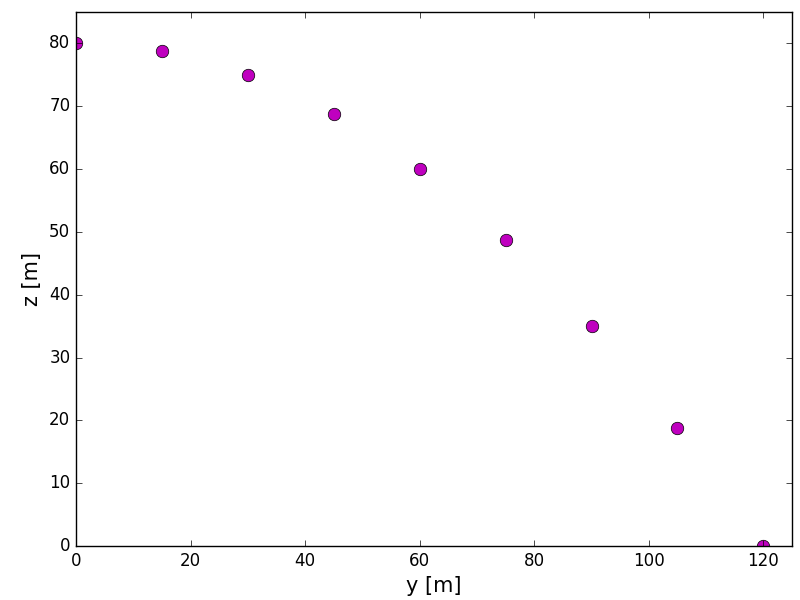
\includegraphics[width=0.5\linewidth]{Kinematika_materijalne_tocke/polozaj_MT.png}
%  \caption{1a}
%  \label{fig:sfig1}
%\end{subfigure}%
%\begin{subfigure}{.5\textwidth}
  \centering
  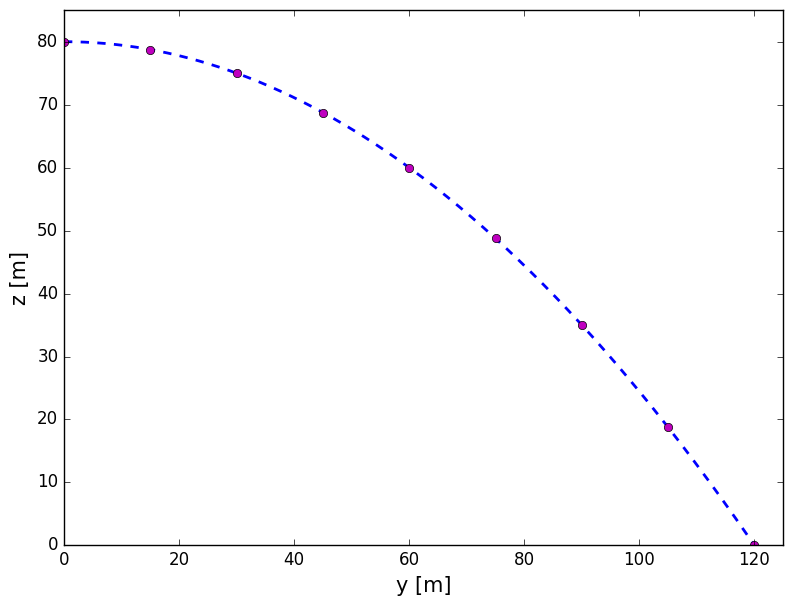
\includegraphics[width=.5\linewidth]{Kinematika_materijalne_tocke/krivulja_MT.png}
%  \caption{1b}
%  \label{fig:sfig2}
%\end{subfigure}
\caption{\textit{(lijevo)} Položaj MT za svakih $0,5\ s$. \textit{(desno)} Putanja MT do udarca o tlo.}
%\label{fig:poloza_MT}
\end{figure}
 
 
 
 \item $$\vec{v}(t)  = \frac{d\vec{r}(t)}{dt}$$
  
 $$\vec{v}(t)  = \frac{d}{dt} \left(z_0 \vec{k}+v_0t \vec{j}-\frac{1}{2}gt^2\vec{k}  \right)$$

 $$\vec{v}(t)  = v_0\vec{j}-gt\vec{k}$$
 
 \item $\vec{v}(t)  =30\ ms^{-1}\vec{j}-10\ ms^{-2}t\vec{k}$
 
 $\vec{v}(t=1s)  =30\ ms^{-1}\vec{j}-10\ ms^{-2}1s\vec{k}$
 
 $\vec{v}(t=1s)  =30\ ms^{-1}\vec{j}-10\ ms^{-1}\vec{k}$
 
 $\vec{v}(t=2s)  =30\ ms^{-1}\vec{j}-20\ ms^{-1}\vec{k}$
 
 $\vec{v}(t=3s)  =30\ ms^{-1}\vec{j}-30\ ms^{-1}\vec{k}$
  
 $\vec{v}(t=4s)  =30\ ms^{-1}\vec{j}-40\ ms^{-1}\vec{k}$
 
\begin{figure}
%\begin{subfigure}{.5\textwidth}
  \centering
  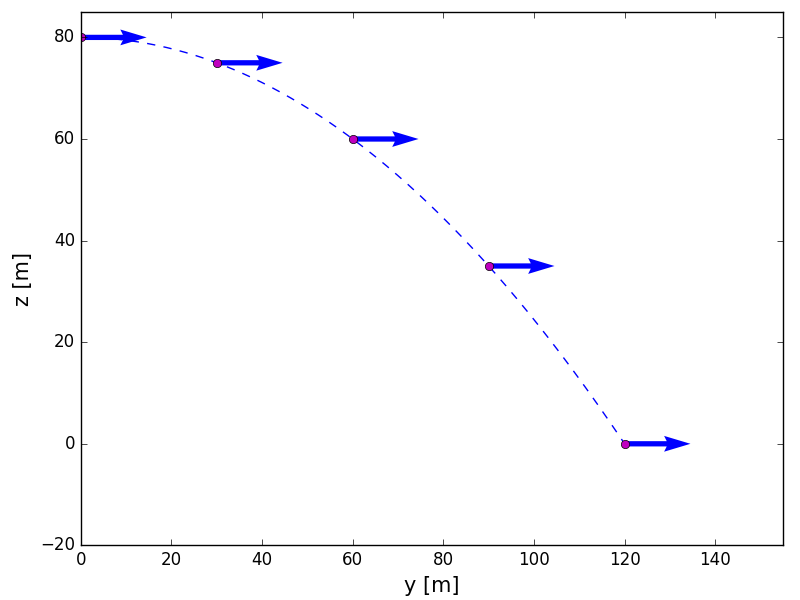
\includegraphics[width=0.4\linewidth]{Kinematika_materijalne_tocke/brzina_y.png}
%  \caption{1a}
%  \label{fig:sfig1}
%\end{subfigure}%
%\begin{subfigure}{.5\textwidth}
  \centering
  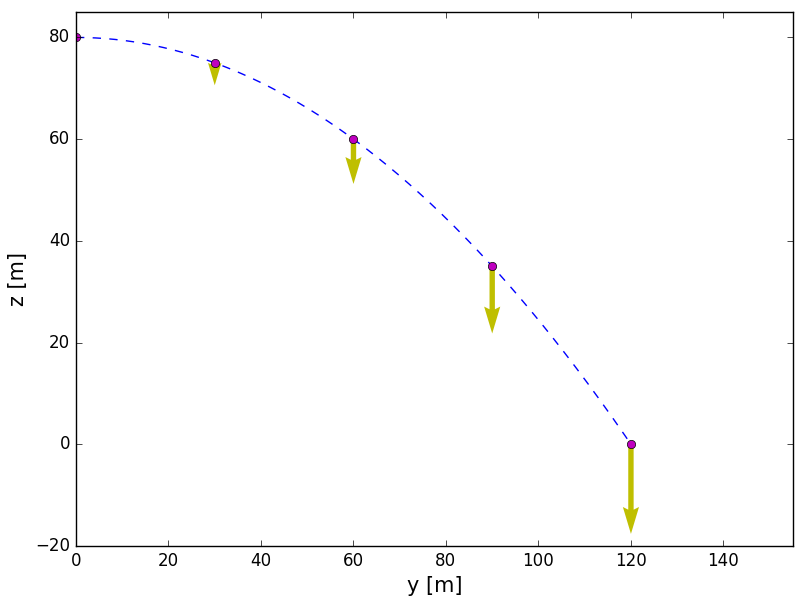
\includegraphics[width=.4\linewidth]{Kinematika_materijalne_tocke/brzina_z.png}
%  \caption{1b}
%  \label{fig:sfig2}
%\end{subfigure}
\centering
  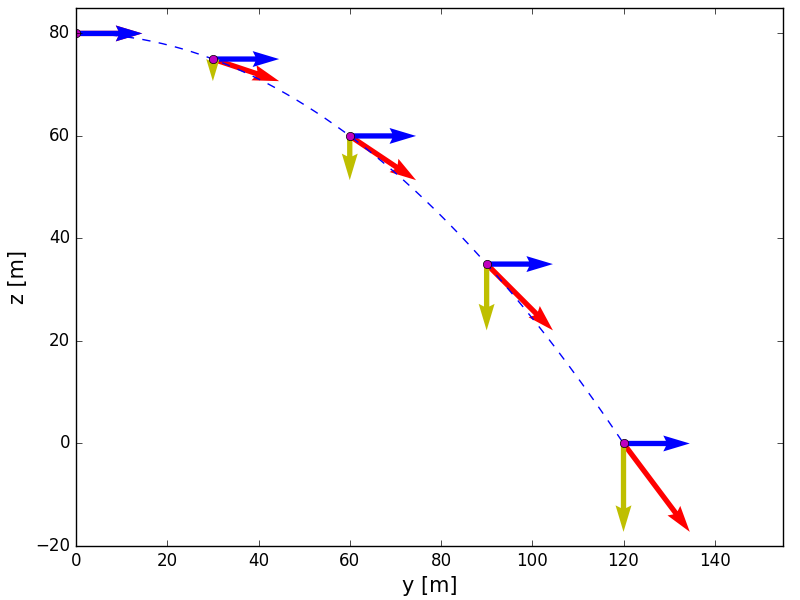
\includegraphics[width=.5\linewidth]{Kinematika_materijalne_tocke/brzina_ukupna.png}
\caption{\textit{(gore-lijevo)} Komponenta brzine u $y$-smjeru. \textit{(gore-desno)} Komponenta brzine u $z$-smjeru.\textit{(dolje)} Brzina tijela s komponentama.}
%\label{fig:brzina}
\end{figure}

$|\vec{v}(t=1s)|  = \sqrt{ (30\ ms^{-1})^2 + (-10\ ms^{-1})^2 } = 31,623\ ms^{-1} $

$|\vec{v}(t=2s)|  = \sqrt{ (30\ ms^{-1})^2 + (-20\ ms^{-1})^2 } = 36,055\ ms^{-1}  $

$|\vec{v}(t=3s)|  = \sqrt{ (30\ ms^{-1})^2 + (-30\ ms^{-1})^2 } = 42,43\ ms^{-1}  $

$|\vec{v}(t=4s)|  = \sqrt{ (30\ ms^{-1})^2 + (-40\ ms^{-1})^2 } = 50,0\ ms^{-1}  $


\item $$\vec{a}(t)  = \frac{d^2\vec{r}(t)}{dt^2}=\frac{d\vec{v}}{dt}$$
$$\vec{a}(t)  = \frac{d} {dt} \left( v_0\vec{j}-gt\vec{k}  \right)$$
$$ \vec{a}(t)  =  -g\vec{k}=-9,81\ ms^{-2}\vec{k}\approx -10\ ms^{-2}\vec{k} $$

\end{enumerate}


{\color{boja} \rule{\linewidth}{0.3mm} }


\begin{enumerate}[label=\alph*)]
 \item U relaciju $\vec{r}(t)$ potrebno je uvrstiti traženo vrijeme
 
 $\vec{r}(t=0,5s)=6\cdot 0,5^4\vec{i}+4\cdot0,5^2\vec{j}+3\cdot0,5\vec{k}$
 
 $ \vec{r}(t=0,5s) = 0,375\vec{i}+1\vec{j}+1,5\vec{k}\ [m] $.
 
 \item  Kako bismo dobili brzinu materijalne točke potrebno je derivirati po vremenu $\vec{r}(t)$
 
 $\vec{v}(t)  = \frac{d\vec{r}(t)}{dt}=\frac{d}{dt}\left( 6t^4\vec{i}+4t^2\vec{j} + 3t\vec{k}  \right) $
 
 $\vec{v}(t) = 24t^3\vec{i}+8t\vec{j}+3\vec{k}  $
 
 $\vec{v}(t=0,5) = 24\cdot0,5^3\vec{i}+8\cdot0,5\vec{j}+3\vec{k}  $
 
 $\vec{v}(t=0,5) = 3\vec{i}+4\vec{j}+3\vec{k}\ [ms] $
 
 $|\vec{v}(t=0,5)| = \sqrt{3^2+4^2+3^2}=5,83\ [ms] $
 
 \item $\vec{a}(t)  = \frac{d^2\vec{r}(t)}{dt^2}=\frac{d\vec{v}}{dt}$
 
 $\vec{a}(t)  = \frac{d}{dt} \left(  24t^3\vec{i}+8t\vec{j}+3\vec{k} \right) $
 
 $ \vec{a}(t)  = 72t^2\vec{i}+8\vec{j}$
 
  $ \vec{a}(t=0,5)  = 72\cdot 0,5^2\vec{i}+8\vec{j}$
  
  $ \vec{a}(t=0,5)  = 18\vec{i}+8\vec{j}$
  
  $ |\vec{a}(t=0,5)|  = \sqrt{ 18^2+8^2}=19,7\ [ms^{-2}]$.
\end{enumerate}


{\color{boja} \rule{\linewidth}{0.3mm} }


Rješavamo inverzni problem i tražimo $\vec{r}(t)=$?
$$
\vec{r}(t)=\vec{r_0}+\int_0^t \vec{v}(\tau)d\tau
$$
$$
\vec{r}(t)=2\vec{i}+3\vec{j}+\int_0^t(4\tau\vec{}i+3\tau^2\vec{j})d\tau
$$
Trebamo riješiti integral $I=\int_0^t(4\tau\vec{}i+3\tau^2\vec{j})d\tau$.
$$
I=\int_0^t 4\tau\vec{}i d\tau + \int_0^t 3\tau^2\vec{j} d\tau= 4\vec{i}\int_0^t \tau d\tau + 3\vec{j}\int_0^t \tau^2d\tau=
$$
$$
=4\frac{t^2}{2}\vec{i}+3\frac{t^3}{3}\vec{j}=2t^2 \vec{i}+t^3\vec{j}
$$
Vratimo se u $\vec{r}(t)$
$$
\vec{r}(t)=2\vec{i}+3\vec{j}+2t^2 \vec{i}+t^3\vec{j}=2(1+t^2)\vec{i}+(3+t^3)\vec{j}
$$
$$
\vec{r}(t=1,2\ s)=2(1+1,2^2)\vec{i}+(3+1,2^3)\vec{j}=4,88\vec{i}+4,728\vec{j}\ \ [m]
$$


 
 



\stepcounter{cjelina} 
\setcounter{zadatak}{0}





%----------------------------------------------------------------------------------------
%	BIBLIOGRAPHY
%----------------------------------------------------------------------------------------

%\bibliographystyle{apalike}

%\bibliography{sample}

%----------------------------------------------------------------------------------------


\end{document}
